\documentclass[12pt]{report}
%\usepackage[francais] {babel} %j'ecis en anglais ,pas besoin de ce package
\usepackage[latin1] {inputenc}
\usepackage[T1] {fontenc}
\usepackage{newcent}
\usepackage{pst-xkey}
\usepackage{pstricks}
\usepackage{pstricks-add}
\usepackage{tkz-tab}
\usepackage{color}
\usepackage{colortbl} % colorer un tableau
\usepackage{url} % insertion de lien cliquable
\usepackage{soul} % soulignement
\usepackage{setspace} % interligne
\onehalfspacing
\usepackage{layout} % marge
\usepackage[top=2cm, bottom=2cm, left=2cm, right=2cm]{geometry}
\usepackage{url}
\usepackage{float} % utile pour inserer les figures cote a cote dans une minipage
\usepackage{soul} % soulignement
\usepackage{mathpazo} % police d'ecriture
\usepackage{ulem} % soulignement
\usepackage{graphicx} % package d'insertion et de manipulation d'image
\usepackage{verbatim} % insertion de codes brut
\usepackage{listings} %insertion de codes brut avec options avance
\renewcommand{\emph}{\textit}
% \usepackage{fancyhdr} realiser des entete et pieds de page personnalise
\lstset
{
	language= R,
	basicstyle=\scriptsize, %taille de la police du code
	numbers=left, %placer le numero de chaque ligne a gauche
	numberstyle=\scriptsize, %taille de la police des numeros
	numbersep=0.5pt, %distance entre la ligne et sa numerotation
	backgroundcolor=\color{grisclaire} % couleur de fond
}
\usepackage{array} % choix des separateurs dans un tableau
\usepackage{amsthm}
\usepackage{amsmath} % packages pour ecriture d'expressions scientifiques
\usepackage{ amssymb} % packages pour ecriture d'expressions scientifiques
\usepackage{mathrsfs} % packages pour ecriture d'expressions scientifiques
\usepackage{array} % choix des separateurs dans un tableau
%\usepackage{slashbox} %  n'est pas encore dans la distribution miktex
%\usepackage{multirow} % n'est pas encore dans la distribution miktex
\usepackage{wrapfig} % insertion d'images cdans un paragraphe
\usepackage{eurosym} %pour l'utilisation du symbole Euro via la commande \euro{}
\newtheorem{theoreme}{Theorem}[section] % insere un "Theoreme" par appelation de l'environnement "theoreme" et numeroté par rapport aux sections
\newtheorem {lemme}{Lemma} % La petite étoile enlève la numérotation, mais nécessite le package amsthm
\newtheorem* {preuve}{proof} % preuves dans l'environnement "proof"
\newtheorem {proposition}{Proposition}[section]  % proposition par appelation de l'environnement "proposition"
\newtheorem {definition}{Definition}[section] % definition par appelation de l'environnement "proposition"
\newtheorem* {definition2}{Definition} % definition par appelation de l'environnement "definition"
\newtheorem{remarque}{Remark}[section]
\newtheorem{corollaire}{Corollary}
\definecolor{grisclaire}{gray}{0.8}

\begin{document}
	
\chapter*{Measurement Error In High-Dimensional Data}
\subsubsection{Abstract}
	{\small \slshape In many important statistical applications, the number of variables (covariates) $p\ $ largely exceed the number of observations (sample size) $n\ $.Such data are refer as high-dimensional data; preceding studies show that some common standard statistical methods of analysis do not conform with this kind of data.Besides, much applied work has been devoted to high-dimensional regression with clean data.However, we often face corrupted data in many applications like in genomic for instance where measurement error cannot be ignored.It is therefore necessarily to highlight some appropriate statistical methods for handling high-dimensional data as well as their extension to the case in which covariates are also mismeasured. The purpose of this study is to introduce reduction of high dimensional data using regularization methods (penalized linear regression) as well as their variants to accommodate  for presence of measurement errors in covariates. In this paper, we evaluate four penalization methods ; ridge regression, Lasso, Dantzig selector and the Elastic net for model fitting then we present their respective variants to account for measurement error.The evaluation focus on situation relevant for practical applications through both simulated and real examples of high-dimensional data sets.}
\subsubsection{Keywords}
High-dimensional data; measurement error; penalized regression; Lasso; Dantzig Selector; Elastic net; ridge regression; Convex conditional Lasso; Non convex lasso; Matrix Uncertainty Selector.
\section{Introduction}

This paper is about measurement error in high-dimensional data.In recent decades, technological progress has led to a great abundance of data in many scientific fields.For example in genetics, a new framework has been developed, in which the number of variables \textbf{p} is larger than the number of observations \textbf{n} (high-dimensional data).High-dimensional data analysis has had a tremendous growth in popularity and a plethora of methods has been proposed for statistical modelling of, and inference in high-dimensional data.Penalized regression methods such as ridge regression \cite{nref8}, Lasso \cite{nref9} methods and Dantzig selector \cite{nref12} are particularly good in this context.

In almost all disciplines, it may not be possible to observe a variable accurately, for some reason, and therefore it is necessary to work with an error-prone version of that variable.Any measurement process can be affected by errors, usually due to the measuring instrument or the sampling process.The consequences of ignoring measurement error, many of which have been known for some time, can range from the non-existent to the rather dramatic.Throughout this work, attention is given to the effects of measurement error on analyses that ignore it. This is mainly because the majority of researchers do not account for measurement error, even if they are aware on its presence  and potential impact.In part this is because the information or extra data needed to correct for measurement error may not be available.Typically , when measurement error creep into the data, there are tree main reason why measurement error cannot be ignored; it can cause bias in parameter estimation \cite{nref1}, interfere with variable selection \cite{nref17} and lead to a loss of power \cite{nref11} leading to trouble in detecting relationships among variables.Results on the bias of naive estimators often provide the added bonus of suggesting a correction method.

Applying high-dimensional regression methods that do not correct for measurement errors result in faulty inference as demonstrated for the Lasso \cite{nref6}. Consequently, correction for measurement error in penalized regression has recently been studied by various authors.Example include ; "Ridge regression approach to measurement error"\cite{nref6} , Non Convex Lasso (NCL) by Loh and Wainwright \cite{nref17}, the Convex Conditional Lasso (CoCoLasso) of Datta and Zou \cite{nref18} and the Matrix Uncertainty Selector proposed by Rosenbaum and Tsybakov (MUS) \cite{nref23}.

The organization of this paper is as follows; \textbf{section 0.2} and \textbf{0.3} presents high-dimensional data together with potential challenges when analysing the later, along with some statistical methods one may use to handle this kind of datasets. \textbf{section 0.5} introduces the measurement error in regression theory, provides an overview of the consequences of measurement error in linear regression and introduces some corrections methods. \textbf{section 0.6} describes behaviour of measurement error in high-dimensional regression and introduces some high-dimensional approaches (methods) to correct for measurement error in high-dimensional context. Both real and simulated data are used for illustrations.

	\section{Introduction to High-Dimensional Data}
\paragraph*{}
High-dimensional data are defined as data in which the number of features (\emph{variables observed}) \textbf{p}, are close to or large than the number of observations (or \emph{data points}) \textbf{n}. The opposite is \textbf{low-dimensional data}, in which the number of observations \textbf{n}, far outnumbers the number of feature \textbf{p}.

A related concept is \textbf{Wide data} which refers to data with numerous features irrespective of the number of observations; similarly, \textbf{tall data} is often used to denote data with large number of observations. This concept should not be therefore confuse with notion of \textbf{big data} which is data that contains greater \textit{variety}, arriving in increasing \textit{volumes} and with more \textit{velocity} known as the threes \textbf{Vs} (visit, \url{https://www.oracle.com/big-data/what-is-big-data/}).

High-dimensional datasets are become more common in many scientific fields as new automated data collection techniques have been developed.And example in biological sciences may include \textit{data collected from hospital patients recording symptoms, blood test results, behaviours and general health} resulting in datasets with large number of features.\\
And example of what high-dimensional data might look like in a biomedical study is shown in figure \ref{tab1} below.
\begin{figure}[h!]
	\begin{center}
		\includegraphics[scale=1]{high.png}
	\end{center}
	\caption[An high-dimensional dataset.]{an overview of an high-dimensional dataset  with P=20011  features and n=200 observations}
	\label{tab1}
\end{figure}
Here are examples of descriptions of research questions whose associate datasets can be considered as high-dimensional data:
\begin{itemize}
	\item predicting patient blood pressure using: \textit{cholesterol level in blood,age and BMI as well as information on 200000 single nucleotide polymorphisms from 100 patients}
	\item Predicting probability of a patient's cancer progressing using: \textit{gene expression data from 20000 genes as well as data associated with general patient health (age, weight,BMI, blood pressure) and cancer growth (tumour , localised spread,blood test results)}
\end{itemize}
Example of application, including in social science are extremely numerous; see \textbf{Plomin (2018)}.
\subsection{Challenge when Analysing High-dimensional Data}
\paragraph*{}
Analyses of high-dimensional data require consideration of potential problems that come with having more features than observations.Such datasets pose a challenge for data analysis as standard methods of analysis, such as \emph{least squares linear regression}, are no longer appropriate.Many of the issues that arise in the analysis of high-dimensional data are know in classical approaches, since they apply also when $n>p$ :
these include the role \emph{bias-variance trade-off} and the danger of \textit{over-fitting}.Though these issues are always relevant, they can become particularly important when the number of features is very large relative to the number of observations.
\paragraph*{}
In other to illustrate the need for extra care and specialized technique for regression when $p>n$, we begin by examining what can go wrong if we apply a statistical technique not intended for high-dimensional setting. For this purpose, we examine \textit{least squares regression}.But the same concepts apply to \emph{logistic regression, linear discriminant analysis} and other classical statistical approaches.


	\subsubsection{Setup of Linear Regression Model}

\paragraph*{}
The general form of the multiple linear regression model is as follows:
\begin{equation}
	Y=\mathbb{E}[Y|X] + \epsilon\ =\ \beta_{0}+\beta_{1}X_{1}+...+ \beta_{p}X_{p} + \epsilon
	\label{f1}
\end{equation}
Where $y$ is the dependent variable, $\beta_{0}, \beta_{1},...,\beta_{p}$ are regressions coefficients, and $X_{1},...,X_{p}$ are independents variables in the model; $\mathbb{E}[Y]$ the expectation of the response variable. In the classical regression setting, it is usually assumed that the error term $\epsilon$ follows the $normal\ distribution$ with mean $\mathbb{E}[\epsilon]=0$ and constant variance $Var[\epsilon]=\sigma^{2}$.

We consider  a datasets from the following model
\begin{equation}
	Y_{i}=\beta_{0} + \beta_{1}X_{i1}+...+\beta_{p}X_{ip}+\epsilon_{i},\: i=1,...,n
	\label{f2}
\end{equation}

Where $X_{ij}$ is the $j^{th}$ variable for individual $i$ and $\epsilon_{i}'s$ are random errors assuming $\mathbb{E}[\epsilon_{i}]=0$ and $Var[\epsilon_{i}|X]=\sigma^{2}\ for\ i=1,2,...,n$. The data from this model can be written in matrix form:
\begin{equation}
	y=X\beta + \epsilon ,
	\label{lrm}
\end{equation}
where: 
$$ y=
\begin{pmatrix}
	y_{1} \\
	\vdots \\
	y_{n}
\end{pmatrix}, \;X= \begin{pmatrix}
	1&x_{11}&x_{12}& \cdots & x_{1p} \\
	1 & x_{21} & x_{22} & \cdots & x_{2p} \\
	\vdots& \vdots&        &         & \vdots \\
	1 & x_{n1} & x_{n2} &   \cdots & x_{np}
\end{pmatrix} ,\; \beta=
\begin{pmatrix}
	\beta_{0} \\
	\vdots\\
	\beta_{p}
\end{pmatrix}, \; and\  \epsilon=
\begin{pmatrix}
	\epsilon_{1}\\
	\vdots \\
	\epsilon_{n}
\end{pmatrix}$$

The regression parameter are estimated by minimizing ordinary least squares:
$$  \sum_{i=1}^{n}[y_{i}-(\beta_{0} + \beta_{1}X_{i1}+...+\beta_{p}X_{ip})]^{2}= (y-X\beta)^{t}(y-X\beta)=\parallel y-X\beta\parallel ^{2},\; (\parallel. \parallel \footnote{$\parallel.\ \parallel$ is the Euclidian norm on $\mathbb{R}^{n}$}).$$
	\subsubsection {Ordinary Least Squares Estimates (OLS Estimates)}
\begin{proposition}[ \textit{from \cite{ref4}} ]
	The least squares estimation of $\beta$ for linear regression model is given by,
	\begin{equation}
		b=argmin_{\beta} \bigg\{\parallel y-X\beta\parallel ^{2}_{2} \bigg\}= (X^{t}X)^{-1}X^{t}y,
		\label{f3}
	\end{equation}
\end{proposition}

assuming $(X^{t}X)$ is a non-singular matrix.Note that this is equivalent to assuming that the matrix $X$ is of full rank\footnote{i.e, $rank(X)=p+1<n$, this then implies that $rank(X^{t}X)=p+1$ and therefore that $X^{t}X$ is invertible.}.\\
The estimator $b=(X^{t}X)^{-1}X^{t}y$ is and unbiased estimator of $\beta$. In addition,its covariance matrix is given by,
\begin{equation}
	 Cov(b)=(X^{t}X)^{-1}\sigma^{2}.\label{10}
\end{equation}
\begin{proposition}[ \textit{ from \cite{ref4}} ]
	The unbiased estimator of the variance $\sigma^{2}$ in the multiple linear regression is given by:
	\begin{equation}
		s^{2}=\frac{RSS}{n-p-1}=\frac{1}{n-p-1}\sum_{i=1}^{n}(y_{i}-\hat{y_{i}})^{2}.
		\label{f4}
	\end{equation}
\end{proposition}
	The proof is straightforward using the following lemmas:
\begin{lemme}
	Let $A_{n\times n}$ be and idempotent matrix of rank $p$ then the eigenvalues of $A$ are either $1$ or $0$.
\end{lemme}
	\begin{lemme}
	If $A$ is and idempotent matrix, then $tr(A)=rank(A)=p$.
\end{lemme}
	\begin{lemme}
	Let $y^{t}=(y_{1},y_{2},...,y_{n})$ be an $n\times 1$ vector with mean $\mu^{t}=(\mu_{1},...,\mu_{n})$ and variance $\sigma^{2}$  for each component. Further, it is assumed that $y_{1},y_{2},...,y_{n}$ are independent.Let $A$ be and $n\times n$ matrix.
	
	The expectation of the quadratic form of random variables is given by:
	\begin{equation}
		\mathbb{E}[y^{t}Ay]=\sigma^{2}tr(A)+\mu^{t}A\mu ,
		\label{f5}
	\end{equation}
\end{lemme}
	Now that a brief presentation of the linear model has been made, come back to the main question to know the problems encountered in high-dimension setting.
\begin{description}
	\item[Theoretically:] When $\ p>n,\ X^{t}X\ $ is not invertible (or near singular ) and $\ s^{2}\ $ in \eqref{f4} is not defined.
\end{description}
	\begin{lemme}
	An $n\times n$ ill-conditioned or near singular matrix has at least one of its eigenvalues close to zero, and then the eigenvalue of the inverse tend to be very large.
\end{lemme}	 
\begin{proposition}[ \textit{ from \cite{ref4}} ]
	The  average Euclidean distance measure $\mathbb{E}[\parallel b-\beta \parallel^{2}]$ between the least squares estimate $b$ and the true parameter $\beta$ is given by:
	\begin{equation}
		\mathbb{E}[\parallel b-\beta \parallel^{2}]=\sigma^{2}tr[(X^{t}X)^{-1}]
		\label{f8}
	\end{equation}
\end{proposition}
	\begin{remarque}
	Assuming that $(X^{t}X)$ has $k$ distinct eigenvalues $\lambda_{1},...,\lambda_{k}$ , then the eigenvalues of $(X^{t}X)^{-1}$ are $\frac{1}{\lambda_{1}},...,\frac{1}{\lambda_{k}}$, denoting by $ V=(v_{1},...,v_{k})^{t}$ the corresponding normalized eigenvectors, we can write $V^{t}(X^{t}X)^{-1}V=D=diag(\frac{1}{\lambda_{1}},...,\frac{1}{\lambda_{k}})$.\\ Moreover, $tr(X^{t}X)^{-1})=tr(V^{t}V(X^{t}X)^{-1})=tr(V^{t}(X^{t}X)^{-1}V)=tr(D)=\sum_{i=1}^{k}\frac{1}{\lambda_{i}}$ ; we then have:
	\begin{equation}
		\mathbb{E}[\parallel b-\beta \parallel^{2}]=\sigma^{2}\sum_{i=1}^{k}\frac{1}{\lambda_{i}}\  \Leftrightarrow\ \mathbb{E}[\parallel b \parallel^{2}]=\parallel \beta \parallel^{2} + \sigma^{2}\sum_{i=1}^{k}\frac{1}{\lambda_{i}}.
		\label{f9}
	\end{equation}	
\end{remarque}

Now it is easy to see that if one of $\lambda_{i} ,\ i=1,...,k$ is very small, say for instance $\lambda_{i}=0.00001$ then roughly, $\parallel b \parallel^{2}=\sum_{i=1}^{k}b_{i}^{2}$ may \textbf{over estimate} $\parallel \beta \parallel^{2}=\sum_{i=1}^{k}\beta_{i}^{2}$ by $10000\sigma^{2}$ times.\newline
The above discussions indicate that if some columns in $X$ are highly correlated with other column in $X$ then, from \textit{lemma(4)} , the covariance matrix $Cov(b)=(X^{t}X)^{-1}\sigma^{2}$ will have one or more large eigenvalues so that the mean Euclidean distance of $\mathbb{E}[\parallel b-\beta \parallel^{2}]$ will be inflated.Consequently, this makes the estimation of regression parameter $\beta$ less reliable.Thus the high levels correlation between variable in high-dimensional datasets will have negative impact on least square estimates of regression parameter.

Clearly, alternative approaches that are better-suited to the high-dimensional setting are required.
\section{Some Statistical Suitable Methods for Handling\\ High-Dimensional Data}
	\subsection{Ridge Regression}
\label{rre}
Ridge regression is one of the remedial measures for handling severe multicollinearity in least squares estimation.Multicollinearity occurs when the predictors included in the linear model are highly correlate with each other.When this is the case, the matrix $X^{t}X$ tends to be singular or ill-conditioned and hence identifying the least squares estimates will encounter numerical problems.
	\begin{proposition}
	$	\mathbb{E}[\parallel b-\beta \parallel^{2}]	=\sum_{j=1}^{n}	(\mathbb{E}[b_{j}]-\beta_{j})^{2} + \sum_{j=1}^{n}	Var[b_{j}]$
\end{proposition}
	According to "Gauss-Markov" theorem, the least squares approach achieves the smallest variance among all unbiased linear estimates.This however does not necessarily guarantee the minimum \textbf{MSE}.

To better distinguish different type of estimators, let $\hat{\beta}^{LS}$ denote the ordinary least square estimator of $\beta$. We shown that $MSE(\hat{\beta}^{LS})=\mathbb{E}[\parallel \hat{\beta}^{LS}-\beta \parallel^{2}]=\sigma^{2}tr[(X^{t}X)^{-1}]$ \eqref{f8} thus,
$\mathbb{E}[\parallel \hat{\beta}^{LS} \parallel^{2}]=\parallel \beta \parallel^{2} + \sigma^{2}tr[(X^{t}X)^{-1}$ \eqref{f9}; it can be seen that, with ill-conditioned $X^{t}X$, the resultant LSE $\hat{\beta}^{LS}$ would be large in length $\parallel\hat{\beta}^{LS}\parallel$ and associated with inflated standard error ( see \eqref{f9}). This inflated variation would lead to poor model prediction as well.

The Ridge regression is a constrained version of least squares.It tackles the estimation problem by providing biased estimator yet with small variance.
	\begin{theoreme}
	For any estimator $b$, the least squares criterion $	\mathcal{Q}(b)= \parallel y-Xb \parallel^{2}$ can be rewritten as its minimum, reached at $\hat{\beta}^{LS}$ plus a quadratic form in $b$.
		\begin{equation}
		\quad  \mathcal{Q}(b)=\parallel y-Xb \parallel^{2}=\underbrace{\parallel y-X\hat{\beta}^{LS}  \parallel^{2}}_{\mathcal{Q}_{min}}+\underbrace{( \hat{\beta}^{LS}-b)^{t}X^{t}X( \hat{\beta}^{LS}-b)}_{\phi(b)}=\mathcal{Q}_{min} + \phi(b)
		\label{f10}
	\end{equation} 
\end{theoreme}
	contour for each constant of the quadratic form $\phi(b)$ are hyper-ellipsoids centred at ordinary LSE $\hat{\beta}^{LS}$.
		The optimization problem in Ridge regression can be state as:
	$$ minimize \parallel \beta \parallel^{2}\ subject\ to\ ( \hat{\beta}^{LS}-b)^{t}X^{t}X( \hat{\beta}^{LS}-b)=\phi_{0}\ for\ some\ constant\ \phi_{0}.$$
	The enforced constrain guarantees a relatively small residual sum of squares $\mathcal{Q}(\beta)$ when compared to its minimum $\mathcal{Q}_{min}$.As a Lagrangian problem, it is equivalent to 
	$$ minimizing\ f(\beta) = \parallel \beta \parallel^{2} + \frac{1}{k}[( \hat{\beta}^{LS}-b)^{t}X^{t}X( \hat{\beta}^{LS}-b)-\phi_{0}],\qquad k>0$$
	Where $\frac{1}{k}$ is the multiplier chosen to satisfy the constraint.
	\begin{proposition}[Hoerl and Kennard (1970)]
		The numerical solution of this problem corresponding to the Ridge regression estimator of $\beta$ is,
		\begin{equation}
			\hat{\beta}^{R}=(X^{t}X+k\mathbb{I}_{p})^{-1}X^{t}y
			\label{f11}
		\end{equation}
	\end{proposition}
	An equivalent way is to write the Ridge problem in the penalized or constrained least squares form by :
\begin{equation}
	minimize\  \parallel y- X\beta \parallel^{2}\quad subject\ to\ \parallel \beta \parallel^{2}\leq s\ for\ some\ constant\ s
	\label{u1}
\end{equation}
the Lagrangian problem become
\begin{equation}
	minimizing\ \parallel y- X\beta \parallel^{2}+\lambda\parallel \beta \parallel^{2}
	\label{f12}
\end{equation} 
which yield the same estimator given in \eqref{f11}.The penality parameter $\lambda \geq 0$ controls the amount of shrinkage in $\parallel \beta \parallel^{2}$.The large value of $\lambda$, the greater amount of shrinkage.For this reason, the Ridge estimator is also called the shrinkage estimator. There is one-to-one correspondence among $\lambda,\ s,\ k\ and\ \phi_{0}$.\\
	Let $\lambda_{max} = \lambda_{1} \geq \lambda_{2} \geq...\geq \lambda_{p}=\lambda_{min}$ denote the eigenvalues of $X^{t}X$, then the corresponding eigenvalues of $Z$ are $\frac{\lambda_{j}}{\lambda_{j} + k},\ j=1,...,p$. From \eqref{f9}, $MSE(\hat{\beta}^{LS})=\sigma^{2}\sum_{j=1}\frac{1}{\lambda_{j}}$.
\begin{proposition}
	If $MSE(\hat{\beta}^{R},k)$ denote the mean square error of ridge regression estimator, then 
	\begin{equation}
		MSE(\hat{\beta}^{R},k)=k^{2}\beta^{t}(X^{t}X+k\mathbb{I})^{-2}\beta +\sigma^{2}\sum_{j}\frac{1}{\lambda_{j}} .	\frac{\lambda_{j}^{2}}{(\lambda_{j}+k)^{2}}=\lambda_{1}(k)+\lambda_{2}(k).
		\label{f17}
	\end{equation}
\end{proposition}
	\begin{theoreme}[ \emph{Hoerl and Kennard (1970)}]
	There always exists a $k > 0$ such that, 
	$$MSE(\hat{\beta}^{R},k)<MSE(\hat{\beta}^{R},0)=MSE(\hat{\beta}^{LS})$$
\end{theoreme}
	\subsection{Lasso Regression}
The Lasso (Least Absolute Shrinkage and Selection Operator) is another shrinkage method like Ridge regression, yet with an important and attractive feature in variable selection.

Ridge regression does have one obvious disadvantage; unlike \emph{best subset, forward step-wise,backward step-wise}\footnote{methods used in low-dimension regression to select the most appropriate variables for a best model}, which will generally select models that involve just a subset of variables, Ridge regression will include all $p$ predictors in the final model.The penality $\lambda\parallel \beta \parallel^{2}$  in \eqref{f12} will shrink all of the coefficients towards zero, but it will not set any of them exactly to zero (unless $\lambda=\infty$).This may not be a problem for prediction accuracy, but it can create a challenge in model interpretation in setting in which the number of variables $p$ is quite large.Increasing the value of $\lambda$ will tend to reduce the magnitudes of the coefficients, but will not result in exclusion of any of the variables.

The Lasso is a relatively recent alternative to Ridge regression that overcomes this disadvantage .The Lasso estimator of $\beta$ is obtained by 
\begin{equation}
	minimizing\  \bigg \{\parallel y- X\beta \parallel^{2}_{2}\bigg\}\quad subject\ to\ \sum_{j=1}^{p}|\beta_{j}|\leq s\ for\ some\ constant\ s
	\label{u2}
\end{equation}
Namely, the $L_{2}$ penality $\parallel \beta \parallel^{2}=\sum_{j=1}^{p}\beta_{j}^{2}$ in Ridge regression is replaced by the $L_{1}$ penality $\parallel \beta \parallel_{1}=\sum_{j=1}^{p}|\beta_{j}|$ in Lasso. The Lagrangian problem become:
\begin{equation}
	minimize_{\beta \in \mathbb{R}^{p} } \{ \parallel y- X\beta \parallel^{2}+ \lambda \parallel \beta \parallel_{1}\}.
	\label{f18}
\end{equation}
	\subsubsection{Computation of Lasso Solution}
The Lasso problem is a convex program, specifically a quadratic program (\textbf{QP}) ( \textsl{visit \cite{ref2} for more detail.}) with a convex constraint.As such, there are many sophisticated \textbf{QP} methods for solving the Lasso. However, there is a particularly simple an effective computational algorithm, that gives insight into how the Lasso works. The Lagrangian form \eqref{f18}is especially convenient for numerical computation of the solution.
	\subsubsection{Theoretical properties of Lasso penalty}
\label{tpl}
A common assumption of Lasso model is \textbf{sparsity}, i.e only a small number of covariates influence the outcome.

Let $S=\big\{j:\beta_{j}\neq 0\big \}$ the index set of non-zero components of the true coefficient vector $\beta \in \mathbb{R}$ and denote the number of relevant covariate by $s=card\{S\}$.Under sparsity assumption, most components of $\beta$ are zero such that $s\ll p$.For any $\lambda\geqslant 0$ define the active set of the Lasso, $\hat{S}(\lambda)=\big\{j:\hat{\beta}_{j}(\lambda)\neq 0\}$.Given $\beta$ ,we order the covariates such that $S=\big\{1,\dots,s\},\ S^{c} =\big\{s+1,\dots,p\big \}$ and considering the partitioning $X=\big(X_{S},X_{S^{c}}\big)$ where $X_{S}\in \mathbb{R}^{n\times s}$ contains the $n$ measurements of the $s$ relevant covariates, and  $X_{S^{c}}\in \mathbb{R}^{n\times(p-s) }$ contains the $n$  measurements of the $(p-s)$ irrelevant covariates.Sample covariance matrix are denote by $\Sigma_{X}$ and the empirical covariance is given by $S_{XX}=\frac{X^{T}X}{n}$.

State the following basic inequality,
\begin{lemme}[\cite{nref14},P.103]
	we have, 
	\begin{equation}
		\frac{1}{n}\parallel X\hat{\beta}^{Lasso}-X\beta \parallel^{2}_{2} +\lambda\parallel\hat{\beta}^{Lasso} \parallel_{1} \leq \frac{2 \epsilon^{t}X(\hat{\beta}^{Lasso}-\beta)}{n}+\lambda \parallel \beta \parallel_{1}.
		\label{f29}
	\end{equation}
\end{lemme}
Now let us introduce the set, $$ \mathcal{A}=\big\{ \frac{2}{n}\parallel \epsilon^{t}X\parallel_{\infty} \leq \lambda_{o}\big\},$$
for a suitable value of $\lambda_{o}$, the set $\mathcal{A}$ has large probability. Indeed, with Gaussian errors this follow from the following lemma:
\begin{lemme}[\cite{nref14}, P.104]
	Suppose that the diagonal elements of the Gram matrix $\frac{X^{T}X}{n}$ equal $1$ for all $j$.Then we have for all $t>0$ and for $\lambda_{0}=2\sigma\sqrt{\frac{t^{2}+2\log(p)}{n}}$,
	\begin{equation}
		\mathbb{P}\big( \mathcal{A}\big)\geq 1-2\exp(-\frac{t^{2}}{2})
		\label{f31}
	\end{equation}
\end{lemme}
\begin{corollaire}[Lasso estimation consistency]
	Let the assumption of lemma \textbf{6} hold. For some $t>0$, let the regularization parameter be $\lambda=2 \hat{\sigma}\sqrt{\frac{t^{2}+2\log(p)}{n}}$ , where $\hat{\sigma}$ is some estimator of $\sigma$. Then with probability at least $1-\alpha$, where $\alpha=2\exp(-\frac{t^{2}}{2})+\mathbb{P}\big(\hat{\sigma}\leq \sigma \big)$.We have:
	\begin{equation}
		\frac{2}{n}\parallel X(\hat{\beta}^{Lasso}-\beta )\parallel^{2}_{2} \leq 3\lambda \parallel \beta \parallel_{1}
		\label{f32}
	\end{equation}
\end{corollaire}
we thus conclude that, taking the regularisation parameter $\lambda$ of order $\sqrt{\frac{\log(p)}{n}}$ and assume that $\parallel \beta \parallel_{1}=o\big(\sqrt{\frac{n}{\log(p)}}\big)$, result in consistency of the Lasso.

This means that , up to the $\log(p)-term$ and compatibility constant $\Phi_{o}^{2}$, the mean squared prediction error is of the same order as if one knew a priori which of the covariates are relevant and using ordinary least squares estimation based on the true relevant $s$ only. 
See also [\textit{Theorem 14.6, Chap 14 from Guedon et al. (2007)}] for the corresponding result for the random design.

Let us define  the vectors $\beta_{S}$ and $\beta_{S^{c}}$ by:
\begin{equation}
	\beta_{j,S}=\beta_{j}\mathbb{1}_{\{j\in S\}},\quad \beta_{j,S^{c}}=\beta_{j}\mathbb{1}_{\{j\notin S\}}. \label{f33}
\end{equation}
Clearly, $\beta=\beta_{S}+\beta_{S^{c}}$ ; $\beta_{S}$ has zeroes outside the index set $S$ and the elements of $\beta_{S^{c}}$ can only be non-zero in the complement $S^{c}$ of $S$.
\begin{definition}[Compatibility condition]
	We say the the compatibility conditionis met for the set $S$ if for some $\Phi_{0}>0$ and for all $\beta \in \mathbb{R}^{p}$ such that $\parallel\beta_{S^{c}}\parallel_{1}\leq 3 \parallel \beta_{S} \parallel_{1}$, it holds that 
	\begin{equation}
		\parallel \beta_{S} \parallel_{1}^{2}\leq \frac{1}{n}\frac{s\parallel X\beta \parallel_{2}^{2}}{\Phi_{o}2^{2}}=\frac{s(\beta^{t} S_{XX}\beta)}{\Phi_{o}^{2}}.
		\label{f34}
	\end{equation}
	
\end{definition}
\begin{theoreme}[\textit{\cite{nref14}, Theorem 6.1,P.107}]
	Suppose the compatibility condition holds for $S$.Then on $\mathcal{A}$, we have for $\lambda\geq 2\lambda_{0}$
	\begin{equation}
		\frac{1}{n}\parallel X(\hat{\beta}^{Lasso}-\beta )\parallel^{2}_{2}+  \lambda\parallel \hat{\beta}^{Lasso}-\beta \parallel_{1}\leq \frac{4 \lambda^{2}s}{\Phi_{o}^{2}}.
		\label{f35}
	\end{equation}
	
\end{theoreme}
\begin{lemme}
	On $\mathcal{A}$, with  $\lambda\geq 2\lambda_{0}$ we have:
	\begin{equation}
		\frac{2}{n}\parallel X(\hat{\beta}^{Lasso}-\beta )\parallel^{2}_{2}+ \lambda \parallel \hat{\beta}^{Lasso}_{S^{c}}\parallel_{1}\leq 3\lambda \parallel \hat{\beta}^{Lasso}_{S}-\beta_{S} \parallel_{1}.
		\label{f36}
	\end{equation}
\end{lemme}
\begin{remarque}
	The theorem combines two results: 
	\begin{equation}
		\frac{2}{n}\parallel X(\hat{\beta}^{Lasso}-\beta )\parallel^{2}_{2}\leq \frac{4 \lambda^{2}s}{\Phi_{o}^{2}}, \quad ( the\ bound\ for\ predictions\ error)
		\label{f37}
	\end{equation}
	\begin{equation}
		\parallel \hat{\beta}^{Lasso}-\beta \parallel_{1}\leq \frac{4 \lambda^{2}s}{\Phi_{o}^{2}}, \quad ( the\ bound\ for\ L_{1}-error\ of\ coefficients\ estimates.)
		\label{f38}
	\end{equation}
\end{remarque}
\begin{corollaire}[estimation accuracy of $\beta$,[\textit{Knight and Fu (2000)}]
	Under compatibility assumptions on design matrix $X$ and on the sparsity $s=card\{S\}$ , for lambda in the suitable range of order $\lambda \thickapprox \sqrt{\frac{log(p)}{n}}$,
	\begin{equation}
		\parallel \hat{\beta}^{Lasso}-\beta \parallel_{1} \overset{\mathbb{P}}{\underset{n\rightarrow +\infty}{\longrightarrow}}0\ ;\quad \parallel \hat{\beta}^{Lasso}-\beta \parallel_{2} \overset{\mathbb{P}}{\underset{n\rightarrow +\infty}{\longrightarrow}}0
		\label{f39}
	\end{equation}
\end{corollaire}
Knowing that Lasso is widely use for model selection, it is necessary to assess how well the sparse model given by Lasso relates to the true model.We make this assessment by investigating Lasso's model consistency (under linear model); That is, for $S=\big\{ j, \beta_{j} \neq 0\big\}$ being the true active set, we look for a Lasso procedure delivering an estimator $\hat{S}=\big\{ j, \hat{\beta}^{Lasso}_{j} \neq 0\big\}$ of $S$ such that $\hat{S}=S$ with large probability.

Since using Lasso estimate involves choosing the appropriate amount of regularization, to study the model selection consistency of the Lasso, we consider two problems: whether there exists a deterministic amount of regularization that gives consistent selection, or for each random realization whether there exists a correct amount of regularization that selects the true model.The so-called \textbf{"irrepresentable condition"} thoroughly interpreted by \textit{Zhao and Yu (2006) \cite {nref15}} is almost necessary and sufficient for both types of consistency.

An estimate which is consistent in term of parameter estimation does not necessarily consistently select the correct model (or even attempt to do so) where the reverse is also true.The former requires $ \hat{\beta}^{Lasso}-\beta \overset{\mathbb{P}}{\underset{n\rightarrow +\infty}{\longrightarrow}}0\ $ while the latter requires $\mathbb{P}\big(\{\hat{S}=S\}\big)\overset{\mathbb{P}}{\underset{n\rightarrow +\infty}{\longrightarrow}}1$. We desire our estimate to have both consistencies. However, to separate the selection aspect of consistency from the parameter estimation aspect.We make the following definitions about \textit{"sign\footnote{$Sign(.)$ maps positive entry to 1 ,negative to -1 and 0 to 0 } consistency"} that does not assume the estimates to be estimation consistent.
\begin{definition}
	An estimate $\hat{\beta}_{n}$ is equal in sign with the true model $\beta$ if and only if,
	$$Sign(\hat{\beta}_{n})=Sign(\beta)$$
\end{definition}
\begin{definition}
	Lasso is strongly sign consistent if there exists $\lambda_{n}=f(n)$, that is , a function  independent of $Y$ and $X$ such that: 
	$$\lim_{n \rightarrow \infty}\mathbb{P}\big(\{ Sign(\hat{\beta}^{Lasso})=Sign(\beta)\}\big)=1,\ (\ast )$$
\end{definition}
\begin{definition}
	Lasso is general sign consistentcy if 
	$$\mathbb{P}\big(\{\exists\lambda \geq 0,Sign(\hat{\beta}^{Lasso})=Sign(\beta) \}\big)=1,\ (\ast \ast)$$
\end{definition}

\begin{remarque}
	\begin{itemize}
		\item Strong sign consistency implies one can use a preselected $\lambda$ to achieve consistent model selection via Lasso.
		\item General sign consistency means for a random realization there exists a correct amount of regularization that select true model.
		\item $(\ast) \Rightarrow (\ast \ast)$
	\end{itemize}
\end{remarque}
\begin{definition}[Irrepresentable Condition]
	We say that , Irrepresentable condition is met for the set $S$ if there exists a constant $\theta \in [0,1[$ such that ,
	\begin{equation}
		\parallel S_{XX}(S^{c},S)S_{XX}(S,S)^{-1}sign\big(\beta_{S}\big)\parallel_{\infty}\leq \theta.
		\label{f40}.
	\end{equation}
\end{definition}

\begin{theoreme}[Variables selection consistency,[\textit{Zao and Yu (2006)}]]
	The irrepresentable condition \eqref{f40} for the active set $S$ is a sufficient and essentially necessary condition for Lasso to select only variables in active set $S$; that is to achieve sign consistency.
\end{theoreme}
\textbf{Proof.} refer to \textit{Zao and Yu (2006) \cite{nref15}} or \textit{Meinshausen and Buhlmann (2010)} for more details.

\begin{remarque}
	The irrepresentable condition , as given in \eqref{f40} depends on the Gram matrix $\frac{X^{t}X}{n}$ but also on the signs of the true unknown parameter $\beta$, whereas the compatibility condition \eqref{f34} only depends on $\Sigma_{X}$.
\end{remarque}

	\subsection{Dantzig Selector (DS)}
The Lasso is not the only $L_{1}-penalization$ possible. from the score equation ,the Dantzig Selector by \textit{Candes and Tao \cite{nref12}} also belongs to the class of regularisation methods in regression.It can be formulated as the Lasso but instead of controlling the squared error loss, it controls the correlation of residuals with $X$.Specifically, the Dantzig selector estimator is defined to be the solution of the minimization problem:
\begin{equation}
	\underset{\beta\in \mathbb{R}^{p}}{min} \big\{\parallel \beta\parallel_{1}\big\}\ subject\ to\ \parallel X^{t}\big(y-X\beta\big) \parallel_{\infty}:=\underset{1\leq i \geq p}{\sup}|\big(X^{t}r\big)_{i}|\leq \lambda_{p}.\sigma,
	\label{f41}
\end{equation}
for some $\lambda_{p}>0,\ where\ r=y-X\beta\ $ is the residual vector.

\begin{remarque}
	The constraint on the residual vector imposes that for each $j\in \{1,\dots, p\}$ , $|\big(X^{t}r\big)_{j}|\leq \lambda_{p}.\sigma$, which guarantees that the residuals are within the noise level.
\end{remarque}

The Dantzig selector and Lasso are closely related.Connections between the Dantzig Selector and the Lasso have been discussed in \textit{Jame et al. (2008)} where it is shown that under some general conditions, the Dantzig Selector and the Lasso produce the same solution path.

Both models share the feature of setting some of parameters to zero i.e they perform variable selection.

\begin{remarque}
	Though under some general conditions , the Lasso and Dantzig may produce the same solution path, they differ conceptually in that the Dantzig stems directly from an estimating equation, whereas the Lasso stems from a likelihood or an objective function.
\end{remarque}
The theoretical results (estimation accuracy and model selection consistency) for the Dantzig selector estimator are provide with detailed supporting proof in [\textit{\cite{nref12}, theorem 1.1; theorem 1.2}]
	\subsection{Elastic-Net Regression}
We ended the section on Lasso regression by saying that it works best when your model contains a lot of useless variables. We also said that Ridge regression works best when most of the variables in your model are useful.

\begin{remarque}
	When we know about all of the parameters in our model, it's easy to choose if we want to use Lasso or Ridge regression; but what do we do when we are in high dimension setting where the model include tons more variables, far too many to know everything about ?.
\end{remarque}

When you have million of parameters, then you will almost certainly need to use some sort of regularization to estimate them.However, the variables in those models might be useful or useless; we don't not in advance.So how do we choose if we should use Lasso or Ridge regression?.

The good news is that we don't have to choose, instead, we use \emph{Elastic-Net} regression. Just like Lasso and Ridge regression, Elastic-Net regression starts with least squares, then it combines the Lasso regression penalty $\lambda_{1}\parallel \beta \parallel_{1}$ with the Ridge regression penalty $\lambda_{2}\parallel \beta \parallel^{2}_{2}$. The Lagrangian problem become 
$$minimize_{\beta}\{\parallel y-X\beta \parallel^{2} +\lambda_{1}\parallel \beta \parallel_{1}+\lambda_{2}\parallel \beta \parallel^{2}\}.$$
Altogether, Elastic-Net regression combines the strengths of Lasso and Ridge regression. Note that the Lasso and Ridge regression penalty get their own $\lambda's$ ; $\lambda_{1}$ for Lasso and $\lambda_{2}$ for Ridge.But more often, the problem is writing as
$$minimize_{\beta}\{\parallel y-X\beta \parallel^{2} +\lambda(\alpha \parallel \beta \parallel_{1}+(1-\alpha)\parallel \beta \parallel^{2})\},\quad for\ \alpha \in [0,1]\; and\ \lambda \geq 0$$, say
\begin{equation}
	\hat{\beta}^{E}(\lambda,\alpha)=argmin_{\beta}\{\parallel y-X\beta \parallel^{2} +\lambda(\alpha \parallel \beta \parallel_{1}+(1-\alpha)\parallel \beta \parallel^{2})\}.
\end{equation}
We still have the regularization parameter $\lambda$ , but we only have one regularization parameter common to both terms, we also have a parameter $\alpha$  which will control the mix between  $L_{1}$ and $L_{2}$ regularization. 
\begin{remarque}
	We notice that:
	\begin{itemize}
		\item $\hat{\beta}^{E}(\lambda,1)=\hat{\beta}^{Lasso}(\lambda),\quad \hat{\beta}^{E}(\lambda,0)=\hat{\beta}^{R}(\lambda),\quad \hat{\beta}^{E}(0,\alpha)=\hat{\beta}^{LS}$
		\item and when $\alpha \notin\{0,1\} $ and $\lambda \neq 0$ , then we get the hybrid of Ridge and Lasso estimation.
	\end{itemize}
\end{remarque}
\subsubsection{Cross-validation to find the best value of $\lambda$}
There are various methods to select the "best" value for $\lambda$. One is to split the data into \textbf{K} chunks. We then use \textbf{K-1} of this as a training set, and the remaining 1 chunk as the test set.We can repeat this until we've rotated through all \textbf{K} chunks, giving us a good estimate of how well each of the lambda values work in our data.This is called \emph{cross-validation}, and doing this repeated \emph{test/train} split gives us a better estimate of how generalisable our model is.

We can use this new idea to choose a lambda value, by finding the lambda that minimises the error across each of the test and training splits.

Let $(X_{k},y_{k})$ denote the subset of $X$ and $y$ for the $k-th$ fold, with $k=1,\dots, K$.The optimal $\lambda$ is obtained by minimizing the total \textit{Cross-validation} error: 
\begin{equation}
	\hat{\lambda}=\underset{\lambda}{argmin}\bigg\{\underbrace{\frac{1}{K} \sum_{k=1}^{K}\frac{1}{n_{k}}\parallel y_{k}-X_{k}\hat{\beta}_{k}(\lambda)\parallel_{2}^{2}}_{CV_{(K)}} \bigg\},
	\label{f42}
\end{equation}
\section{Numerical Implementation}
{\small We present here two illustrative numerical applications. The first one is based on simulated data and the last one on real data.The purpose of the numerical experiment is to show the behaviour and to investigate if there was an difference in predictive power between the previous three regularization methods; ridge, Lasso and Elastic-net regression when they were applied on high-dimensional data.The statistical analysis was implement using \textbf{R} statistical software.
	\subsection{Simulated Data}
	For the simulation study, we use generalized linear model (GLMs) for penalized logistic regression.The "\textit{glmnet}" \cite{nref28} package for \textbf{R} fits a GLM via penalized maximum likelihood. We will not provide a theory about GLMs in this study ; for specific information regarding GLMs we refer to \cite{nref29} .The measures that are used to assess how good a logistic regression model is for prediction are : \textit{misclassification error rate }(ME) which denotes the fraction of incorrect classifications over all observations and the \textit{Area Under Curve} (AUC) which is a measure of discrimination tanking values between 0 and 1 (visit \cite{nref30} for more details).The simulation study was inspired by the paper by \textit{Krona } \cite{nref30}. However, adjustments were made to the simulated datasets.
	\paragraph{Process description :}
	The simulated data consisted of four independent high-dimensional datasets.Each dataset was divided into a training and a test set.The three methods were used to fit a corresponding model to each of the training sets.The fitted models were used to make predictions for each of the corresponding test sets.Finally, we computed the AUC , the ME and extracted the number of non-zero $\hat{\beta}$-coefficients.The procedure was repeated 100 times per example.
	\paragraph{Simulation design :}
	We simulated p=1000 predictor and n=200 observation such that $p>>n$ and the data qualified as high-dimensional. All predictor variables $X$ were continuous multivariate normal distributed except for the binary response variable $Y$. A multiple group of predictors with varying strength of correlation were simulated for each data set. The predictors were generated by sampling from a multivariate normal distribution with the following probability density function :
	$$ f_{X}(x)=\frac{1}{(2\pi)^{\frac{n}{2}} \sqrt{\det\big(\Sigma\big)}}\exp\bigg\{-\frac{1}{2}(x-\mu)^{t}\Sigma^{-1}(x-\mu)\bigg\}$$  
	were $\mu$ is the mean vector and $\Sigma=(\rho_{ij})_{i,j}$  is the covariance matrix.For all $x$, we set $\ \mu=0\ $ and $\ Var[x]=1\ $.Thus, $\Sigma\ $ equal the correlation matrix of X. Each predictor variable was assigned a predetermined $\ \beta-value\ $.The response variable were simulated by running the simulated data through the inverse logit function ( see \cite{nref29}) ,
	$$\pi(x)=\frac{1}{1+e^{-X^{t}\beta}}.$$
	Given the threshold $\pi_{0}=0.5$, the observed value was categorized into one of the two classes $\ Y=1\ $ if $\ \pi(x)>0.5\ $ and $\ Y=0\ $ if $\ \pi(x)\leq0.5$ .Consequently, we obtained a vector Y and a matrix X consisting of 200 observations of the binary response variable and the predictor variables respectively.
	\paragraph{Details information about the four examples :}
	\begin{description}
		\item[Example 1 :] we set the pairwise correlation between $\ X_{i}\ and\ X_{j}\ $ predictors to $\ \rho_{ij}=0.5^{|i-j|}\ $. We assigned the first 122 $\beta$-coefficients a specified vector that consisted of random values within [2,5].The remaining coefficients were set to 0.
		\item[Example 2 :] we set $\ \rho_{ij}=0.5^{|i-j|}\ $. we set all coefficients to be $\beta=0.8$.
		\item[Example 3 :] we set $\ \rho_{ij}=0.9^{|i-j|}\ $. The coefficients were split in 8 groups, where the coefficients were set to pairwise be 0 and 2, $\beta=(\underbrace{2,2,\dots,2}_{125},\underbrace{0,0,\dots,0}_{125},\underbrace{2,2,\dots,2}_{125},\dots)^{t}$.
		\item[Example 4] The pairwise correlation between the first 500 predictors $\ X_{i}\ and\ X_{j}\ $ ( $\ 1\leq i,j \leq 500\ $) were set to $\ \rho_{ij}=0.5^{|i-j|}\ $ and the pairwise correlation for the remaining predictors were set to 0.We set the first 500 coefficients to $ \beta=3 $ and the remaining coefficients to 0, $\beta=(\underbrace{3,3,\dots,3}_{500},\underbrace{0,0,\dots,0}_{500})^{t}$.
\end{description} }

\paragraph{Results :}
\begin{table}[b]
	\begin{center}
		\begin{tabular}{|c|c|c|c|c|c|c|}
			\hline
			models & \multicolumn{3}{c|}{\textbf{Example 1}}&\multicolumn{3}{c|}{\textbf{Example 2}}\\
			\hline
			&AUC&ME&Nb. of $\hat{\beta}\neq 0$& AUC & ME & Nb. of $\hat{\beta}\neq 0$ \\
			\hline
			Ridge& 0.76 (0.042) & 0.32 (0.053)  & 1000   & 0.76 (0.050) & 0.31 (0.052)  &1000  \\
			
			Lasso&0.65 (0.106)  & 0.41 (0.094)  & 29  & 0.55 (0.058) & 0.46 (0.056)  & 20\\
			
			Elastic Net& 0.75 (0.062) & 0.37 (0.074)  & 316  & 0.70 (0.076) & 0.37 (0.068)  &329 \\
			\hline
			& \multicolumn{5}{c }{ }&  \\
			\hline
			& \multicolumn{3}{c|}{\textbf{Example 3}}&\multicolumn{3}{c|}{\textbf{Example 4}}\\
			\hline
			models&AUC&ME&Nb. of $\hat{\beta}\neq 0$ & AUC & ME & Nb. of $\hat{\beta}\neq 0$ \\
			\hline
			Ridge& 0.92 (0.028) &0.16 (0.041)   &1000   & 0.76 (0.047) & 0.31 (0.041)  & 1000 \\
			
			Lasso&0.84 (0.037)  & 0.24 (0.048)  & 54  &0.58 (0.073)  & 0.46 (0.070)  & 21\\
			
			Elastic Net&0.90 (0.033)  &  0.17 (0.045) & 415  & 0.70 (0.059)  &0.36 (0.054)   & 361 \\
			\hline
		\end{tabular}
	\end{center}
	\caption[Simulation results]{Simulation results.\textit{The table reports the AUC, ME-values and number of non-zero $ \hat{\beta}-coefficients\ $.The simulation was repeated 100 times for each example and all results are reported as median values and (standard deviation sd.)}}
	\label{tab4}
\end{table}
{\small The simulation of Example 1-4 was repeated 100 times: for every simulation, we calculated AUC, ME and their standard deviations (sd).In addition, the average number of selected variables by Lasso and  the Elastic net was calculated.The results are summarized in table \ref{tab4}.
	
	In example 1, a small subset of predictors were assigned non-zero $\ \beta$-coefficients.On average, the Lasso and the elastic net  selected 28 and 316 variables respectively. We  see that the Ridge regression has the highest AUC and the lowest ME.
	
	In example 2, the predictors were assigned coefficients $\ \beta$=0.8 with relatively high correlation amount predictors.As demonstrate in table \ref{tab4}, ridge regression improve over other methods considering AUC and ME. As mention in \textit{subsection 1.3.1}, ridge regression tend to perform well under the circumstances in example 2.Moreover, the average number of coefficients for Lasso and elastic net was 20 and 328 respectively.In this setting, the elastic-net identify a larger number of coefficients that were correlated and non-zero.The Lasso, on the other hand results in a sparse final model but identify less of the non-zero coefficients.instead, the chosen model resulted in a high ME ( table \ref{tab4}).
	
	In example 3, the predictors were divided into 8 groups and pairwise assigned coefficients of 0 and 2.We see that ridge regression outperform the Lasso and elastic net in view of the AUC.Since the elastic net and ridge regression perform considerably similar, they seem to perform equally as good in this setting.As discussed in earlier , ridge regression included all predictors in the final model and resulted in a less interpretable model.However, the elastic net identified on average 415 non-zero coefficients.supposedly, the elastic net adopted the grouping effect and correctly identified almost all non-zero coefficients simultaneously as it achieved high prediction accuracy.
	
	In example 4, the predictors were divided into two groups of equal size that were assigned with $\ \beta$=3 and $\ \beta$=0 respectively.The first 500 were correlated while the remaining 500 predictors were uncorrelated.As seen in table \ref{tab4} , ridge regression achieved the highest AUC  while elastic net succeeded to identified approximately all non-zero coefficients as a result of the grouping effect.
	\paragraph{Summary}
	The results show that the three methods perform well in the sense that AUC$\geq$0.5 in examples 1-4.We observe that despite the fact that ridge regression tend to spread the coefficients shrinkage over a large number of coefficients, it achieve high predictive power throughout example 1-4.especially, the results in example 3 demonstrated the capacity of ridge regression.We identify that when the number of predictor are very large and a larger fraction of them most be included in the model, ridge regression dominates the Lasso and the elastic net.Consequently, it confirm that ridge regression is satisfactory method for prediction on correlated datasets.The results from example 2 determine that the Lasso is outperformed by the elastic net.Furthermore we observed that the elastic net benefits from the ability to put a larger weight to the quadratic penalty, while it simultaneously shrinks some coefficients to zero by the absolute penalty.
	
	Moreover, we observe that ridge regression and the elastic net generally improve over the Lasso.We can see that elastic net approximately identified all-non zero coefficients in the simulations.In example 4, elastic-net performed grouped selection and showed to be a better variable selection method than Lasso.Even though ridge regression did not incorporate variable selection, it achieved high prediction accuracy through-out example 1-4.Therefore, we observe that if the interpretability is not fundamental, ridge regression manage to accomplish high predictive power.Ultimately, the elastic net has the advantage of incorporating variable selection.Consequently , its final model is more interpretable than that of ridge regression.\\
	\subsection{Real data example}
	\paragraph{Data description:}
	For real data example, we will be working with \textit{"human DNA methylation data"} from \textit{"flow-sorted blood samples"}. DNA methylation assays measure for each of many sites in the genome, the proportion of DNA that carries a methyl mark ( a chemical modification that does not alter the DNA sequence).In this case, the methylation data come in the form of normalised methylation levels (M-values) where negative values correspond to unmethylated DNA and positive values correspond to methylated DNA.Along with this, we have a number of sample phenotypes (e.g BMI, Sex, Age in year).This methylation object is a \textit{"GenomicRatioset"}, a \textit{Bioconductor}\cite{nref31} data object derived from the \textit{"SummarizedExperiment"}\cite{nref32}.These \textit{"SummarizedExperiment"} objects contain  \textit{"assays"}, in this case normalised methylation levels, and optional sample level \textit{"ColData"} and feature-level \textit{"metadata"}.These objects are very convenient to contain all of the information about a dataset in a high-throughput context.For more details on these objects, one could consult the \textit{vignettes on Bioconductor}....url....
	
	After reading in the data we can see in the provided R output that this object has $dim() \ of\ 5000\times37\ $, meaning it has 5000 features and 37 samples ( observations).to extract the matrix of methylation M-values, we use "\textit{assay()" function}.Note that in the matrix of methylation data, samples or observations are stored as rows.
	
	In this episode, we will focus on the association between \textbf{Age} and \textbf{methylation}.
	\paragraph{Experiment steps :} Let's denote by X the methylation matrix,
	\begin{description}
		\item[1) Singularity:] we investigete singularity of the matrix $\ X^{t}X\ $ and check out what happen if we try to fit linear model to the data.
		\item[2) Ordinary least square versus Ridge regression :] here, we work with a set of feature known to be associated with \textbf{Age} from a paper by \textit{Horvath et al.}.Horvath et al. used methylation markers alone to predict the biological \textbf{Age} of an individual.
		\begin{itemize}
			\item we extra the first 20 features of the features identified by Horvath, investigate correlations and we split the methylation data matrix and the age vector into training an test sets.
			\item we fit both linear regression and ridge regression on the training data matrix and training \textbf{Age} vector using the previous features and record the MSE between our predictions and the true \textbf{Age}s for the test data.
		\end{itemize}
		\item[3) Apply egularization methods :] we perform the Lasso, Ridge and Elastic-net on the whole DNA methylation data using cross validation to select the tuning parameter, examine the coefficients paths for each method and load Horvath signature to compare features selected by Lasso and the elastic-net methods.
\end{description}}
\paragraph{Results.}
\begin{itemize}
	{\small	\item[1)] We can see  that we are able to get some effect size estimates, but they seem vert high.The \textit{"Summary"} also says that we were unable to estimate effects sizes for 4964 features because of  singularities.What this mean is that R couldn't find a way to perform the calculations necessary due to the fact that we have more features than observations.
		\item[2)] Preditors are correlated each other.Since we split the data into test and training data, we can see that ridge regression gives us a better prediction on unseen data despite being worse on train data : $MSE_{lm}=45.14 \ \geq\ MSE_{ridge}=25.30 $. \textit{see also comments of Figures 1.4 and 1.5}
	 }

	\begin{figure}[b]
		\begin{minipage}[c]{0.49\textwidth}
			\centering
			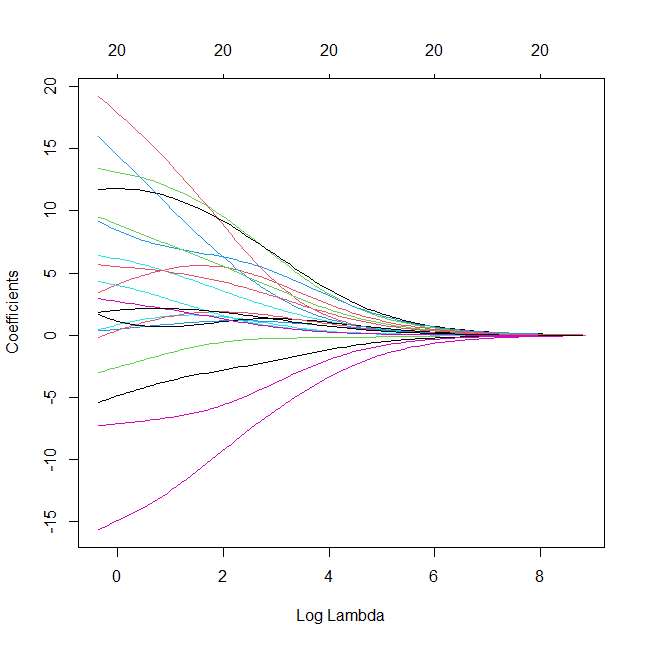
\includegraphics[scale=0.4]{fig1.png}
			
			\caption[plot showing how estimated coefficients for each methylated site change]{\textit{plot showing how estimated coefficients for each methylated site change as we increase the penalty $\ \lambda$. We can see that initially, some parameter estimates are really large, and these tend to shrink fairly rapidly.} }
		\end{minipage}
		\hfill
		\begin{minipage}[c]{0.49\textwidth}
			\centering
			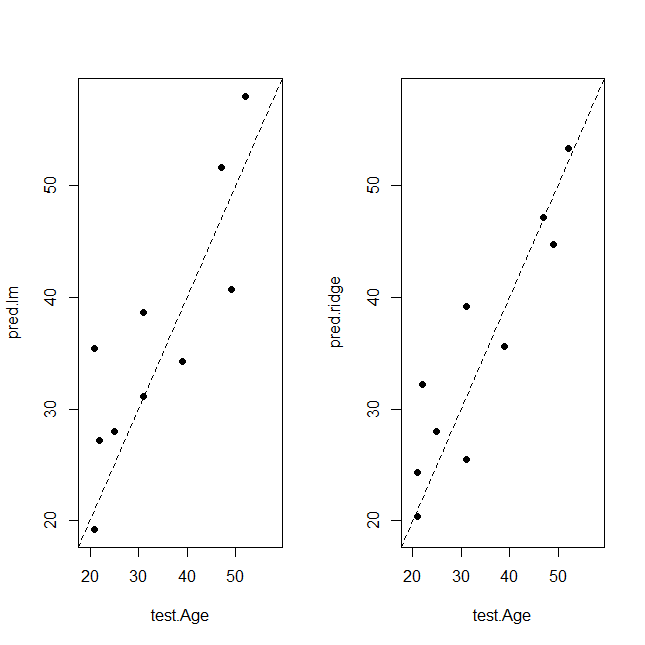
\includegraphics[scale=0.4]{fig2.png}
			\caption[Predicted Ages for each methods against the true Ages]{\textit{Predicted Ages for each methods against the true Ages. The ridge ones are much less spread out with far fewer extreme predictions.}}
		\end{minipage}
	\end{figure}
{\small	\item[3)] Comparing the feature selected by Lasso ( 41 features) and the elastic net ( 60 features ) with Horvath signature, we can see that we selected some of the same feature ( 8 features for Lasso and 11 features for elastic net).\textit{see also the comments of the remaining 6 figures.} }
	\begin{figure}
		\begin{minipage}[c]{0.49\textwidth}
			\centering
			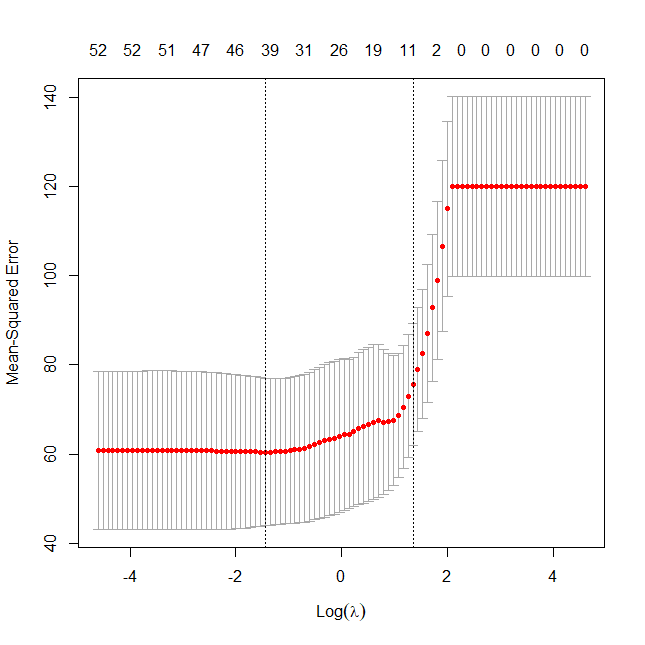
\includegraphics[scale=0.4]{fig3.png}
			
			\caption{\textit{Cross-validation performance for Lasso.}}
		\end{minipage}
		\hfill
		\begin{minipage}[c]{0.49\textwidth}
			\centering
			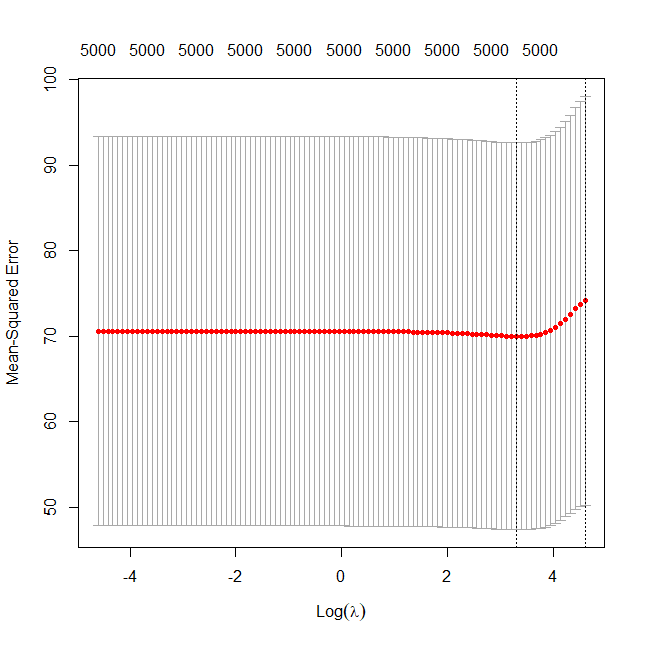
\includegraphics[scale=0.4]{fig4.png}
			\caption{\textit{Cross-validation performance for Ridge.}}
		\end{minipage}
	\end{figure}
	\begin{figure}
		\begin{minipage}[c]{0.49\textwidth}
			\centering
			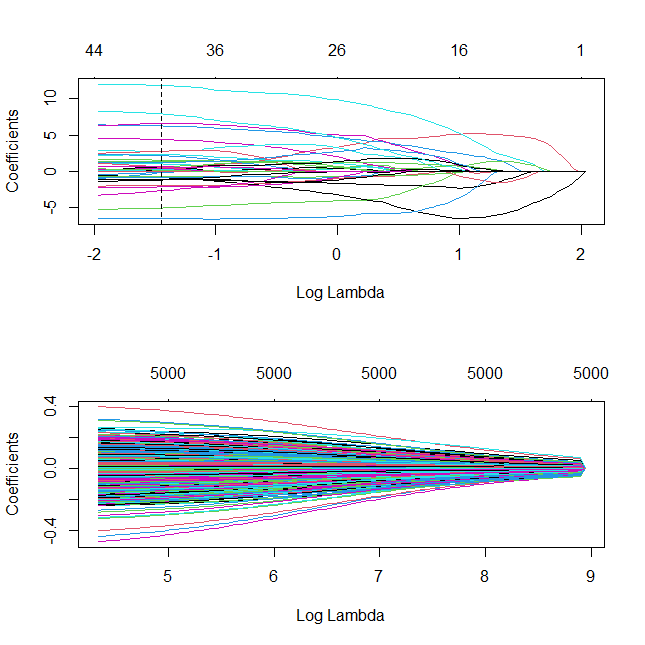
\includegraphics[scale=0.4]{fig5.png}
			
			\caption[Ridge versus Lasso coefficients paths]{\textit{The paths tend to go exactly to zero much more when sparsity increases when we use lasso model.In ridge case, the paths tends toward zero but less commonly reach exactly zero.}}
		\end{minipage}
		\hfill
		\begin{minipage}[c]{0.49\textwidth}
			\centering
			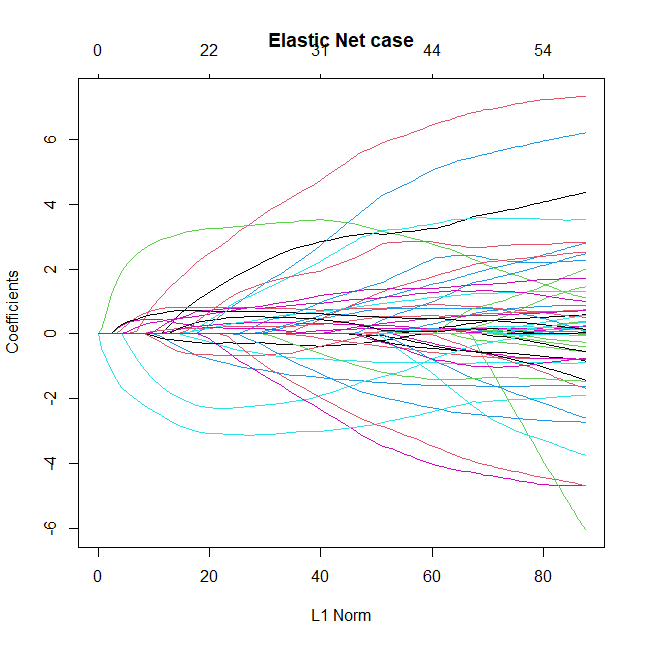
\includegraphics[scale=0.4]{fig6.png}
			\caption[Coefficients paths elastic net]{\textit{Coefficients paths elastic net.We can see that coefficients tend to go exactly to zero, but the paths are a bit less extreme than with pure Lasso; similar to ridge.}}
		\end{minipage}
	\end{figure}
	\begin{figure}
		\begin{minipage}[c]{0.49\textwidth}
			\centering
			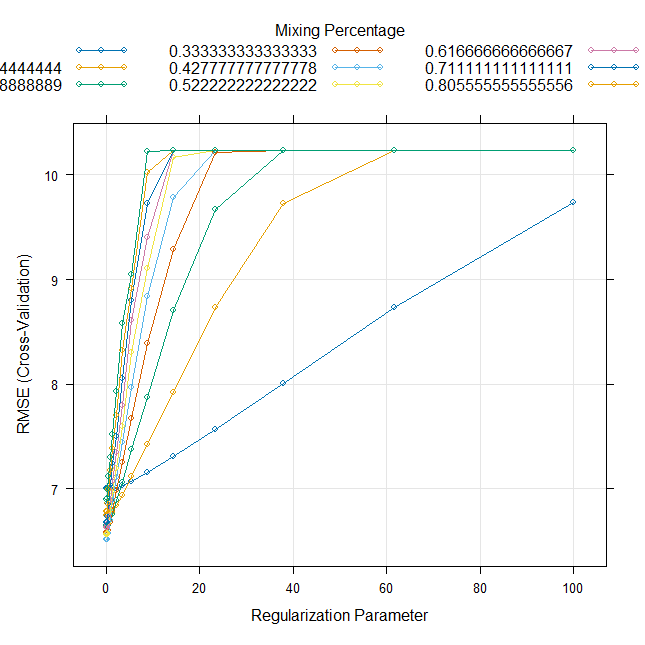
\includegraphics[scale=0.4]{fig7.png}
			
			\caption[Cross-validation for elastic net regression]{\textit{Cross-validation to find the optimal pair of ($\alpha,\lambda\ $) for elastic net (mixing percentage).}}
		\end{minipage}
		\hfill
		\begin{minipage}[c]{0.49\textwidth}
			\centering
			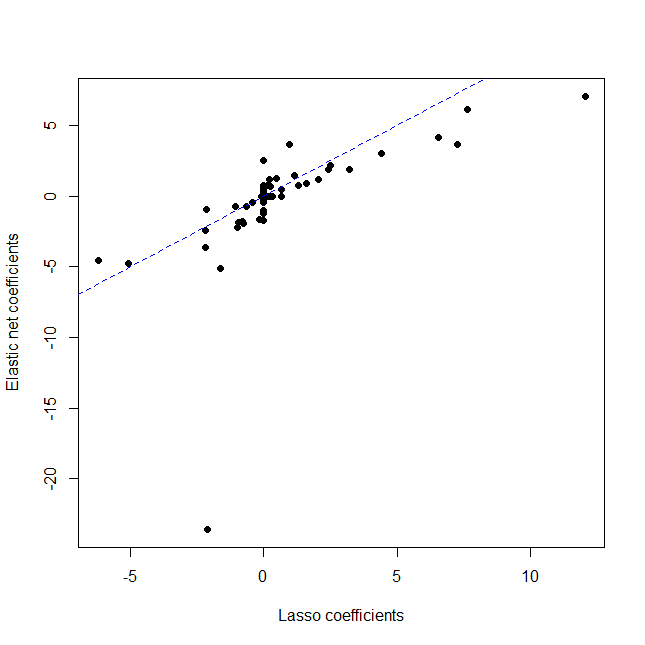
\includegraphics[scale=0.4]{fig8.png}
			\caption[Lasso coefficients against elastic net coefficients]{\textit{Lasso coefficients against elastic net coefficients.We can see that the coefficients from these two methods are broadly similar, but the elastic net coefficients are a bit more conservative.}}
		\end{minipage}
	\end{figure}
\end{itemize}
\section{Measurement Error In Regression theory }
In some sense, all statistical problems involve measurement error.

Measurement error occur whenever we cannot exactly observe one or more of the variables that enter into a model of interest.There are many reason such errors occur, the most common ones being "sampling error and instrument error".Where any notation is used here, the true value is denoted "$X$" and the variable observed in place of "$X$" by "$W$" (error-prone measurement). When the true and observed values are both categorical, then measurement error is more specifically referred to as \textbf{misclassification}.

Measurement error occur in nearly every discipline; Here is a collection of examples in bio-medical field:
\begin{description}
	\item[Genomic:] In recent decades, genetic and epigenetic studies have become increasingly more important in medical research, but the process of sequencing DNA typically involves some errors.
	\item[Disease statut:] I n epidemiology , the outcome variable is often presence or absence of a disease such as breast cancer, hepatitis, AIDS\dots .This is often assessed through an imperfect diagnostic procedure such as an imaging technique or a blood text which can lead to either false positives or false negatives (misclassification).
\end{description}
\subsubsection{Objective and some terminology}
\label{spc}

\begin{itemize}
	\item how to model measurement error ?
	\item what the effects of ignoring it are ?
	\item How, if at all can we correct for measurement error ?
\end{itemize}
These are three general objective in measurement error problem we will try to address in this parts of our work.
\subsubsection{The Model Description}  
One of the fundamental assumption in the linear regression analysis is that all observations are correctly observed.When this assumption is violated the measurement error creep into the data.The the usual statistical tools tend to loose their validity( \textit{see \cite{nref2} and \cite{nref3} for more details.}). And important issue in the area of measurement errors is to find the consistent estimators of the parameters which can be accomplished by using some additional information from outside the sample.

In section \textit{0.6} and \textit{0.7} we consider a linear regression model defined in \eqref{lrm} with additive error,

\begin{equation}
	y=X\beta + \epsilon\ ,\ W=X+U
	\label{f46}
\end{equation}
$X_{i}=(X_{i1},\dots,X_{ip})^{t},\quad W_{i}=(W_{i1},\dots,W_{ip})^{t},\quad U_{i}=(U_{i1},\dots,U_{ip})^{t};$
$$ X=
\begin{bmatrix}
	X_{1}^{t} \\
	\vdots \\
	X_{n}^{t}
\end{bmatrix}\ n\times p\ matrix;\  U=
\begin{bmatrix}
	U_{1}^{t} \\
	\vdots \\
	U_{n}^{t}
\end{bmatrix}\ n\times p\ matrix;\  W=
\begin{bmatrix}
	W_{1}^{t} \\
	\vdots \\
	W_{n}^{t}
\end{bmatrix}\ n\times p\ matrix$$
For the sake of notation simplicity, we assume that $\beta_{0}=0$. The true covariate $X$ are not observed, and instead we have noisy measurements $W=X+U$ where $U$ is and $n\times p$ random noise matrix with covariance matrix $\Sigma_{U}$.If the $k-th$ variable has been measured correctly, the corresponding column of U will be set equal to zero, as will the variance of the measurement error of the $k-th$ variables, $\Sigma_{U(k,k)}=0$.

\textbf{Assumption}
\begin{itemize}
	\item the matrix of measurement error $U \in \mathbb{R}^{n\times p}$ is assumed to have normally distributed rows , with mean zero and covariance $\Sigma_{U}$. 
	\item furthermore, assume that $\epsilon$ and $U$ are independent and  $\Sigma_{U}$ is a $p\times p$ matrix of Known values with non-negative diagonal elements.
\end{itemize}
\begin{remarque}
	It follow from the structural model
	\begin{equation}
		y_{i}=\beta^{t}X_{i}+\epsilon_{i},\ W_{i}=X_{i}+U_{i}
		\label{f47}
	\end{equation} that the vector $\big(y_{i},W_{i}^{t}\big)^{t}$ follows a p+1-variate normal distribution with mean $\mu= \big(\beta^{t}\mu_{X},\mu_{X}^{t}\big)^{t}$ and the covariance matrix,
	\begin{equation}
		\Gamma=\begin{bmatrix}
			\sigma^{2}_{Y}& \Sigma_{YW} \\
			\Sigma_{WY} &\Sigma_{W} \\
		\end{bmatrix} =\begin{bmatrix}
			\sigma^{2}+\beta^{t}\Sigma_{X}\beta& \beta^{t}\Sigma_{X} \\
			\Sigma_{X}\beta &\Sigma_{X}+ \Sigma_{U}\\
		\end{bmatrix}.
		\label{f48}
	\end{equation}
\end{remarque}
This lead to:

\begin{equation}
	y_{i}|W_{i}=w_{i}=\gamma^{t}w_{i}+\delta_{i}
	\label{f49}
\end{equation}
where$\delta=(\delta_{1},\dots,\delta_{n})^{t}$ are i.i.d normally with mean zero and variance $\sigma^{2}_{\delta}$.
\begin{theoreme}
	Under the given assumptions, $\gamma$ and $\sigma_{\delta}^{2}$ are given by,
	\begin{equation}
		\gamma=\big(\Sigma_{W}\big)^{-1}\Sigma_{X}\beta=\big(\Sigma_{X}+\Sigma_{U}\big)^{-1}\Sigma_{X}\beta
		\label{gam}
	\end{equation}
	\begin{equation}
		\sigma_{\delta}^{2}= \sigma^{2}+\beta^{t}\Sigma_{X}\beta-\gamma^{t}\big(\Sigma_{X}+\Sigma_{U}\big)\gamma
	\end{equation}
\end{theoreme}

Thus
\begin{equation}
	\beta=\mathcal{K}_{X}^{-1}\gamma.
	\label{f50}
\end{equation}
where $\mathcal{K}_{X}=\big(\Sigma_{X}+\Sigma_{U}\big)^{-1}\Sigma_{X}$ is a $p\times p$ matrix  referred to as the \textit{reliability matrix} ,\textit{see Gleser (1992) \cite{nref4}  and Aickin and Ritenbaugh (1992)} for example,discussion and illustrations of the role of reliability matrix.

	\subsubsection{Estimated Coefficients and Behaviour of naive analyses}


Statistical analysis that is carried out by ignoring the presence of the measurement error is called a naive approach.
Without measurement error, we saw that the estimated coefficients and the unbiased estimator of $\sigma^{2}$ are given by $\hat{\beta}=(X^{t}X)^{-1}X^{t}y$ \eqref{f3}  and $\hat{\sigma}^{2}=\frac{1}{n-p}\sum_{i}(y-\hat{y}_{i})^{2},\ with\ \hat{y}_{i}=\hat{\beta}^{t}x_{i}$.
\begin{proposition}
	The maximum likelihood estimators of $\gamma$ and $\sigma_{\delta}^{2}$ are just the naive least squares estimators,
	\begin{equation}
		\hat{\beta}_{naive}=\hat{\gamma}=(W^{t}W)^{-1}W^{t}y=S_{WW}^{-1}S_{Wy}\ ,\ \hat{\sigma}^{2}_{naive}=\hat{\sigma}_{delta}=\frac{1}{n-p}\sum_{i}(y-\hat{y}_{i})^{2},\ with\ \hat{y}_{i}=\hat{\beta}^{t}_{naive}w_{i}
		\label{f51}
	\end{equation}
\end{proposition}
where, $S_{WW}=\frac{W^{t}W}{n}$ is the unbiased estimator of $\Sigma_{W}$ and $S_{Wy}=\frac{W^{t}y}{n}$
\begin{proposition}
	The exact bias expression for the naive estimators under the given assumptions are given by:
	\begin{equation}
		\mathbb{E}\big[\hat{\beta}_{naive}\big]=\gamma=\mathcal{K}_{X}\beta \ , \ \mathbb{E}\big[\hat{\sigma}_{naive}^{2}\big]=\sigma^{2}_{\delta }
		\label{f52}
	\end{equation}
	\begin{remarque}
		This result lead to an important conclusion: The measurement error in one of the variables may induce bias in the estimation of all coefficients including those measured without error.If more covariates are affected by measurement error, the resulting bias may become rather complex and the effect of measurement error may become difficult to describe.
	\end{remarque}
\end{proposition}

	\subsubsection{Correcting for Measurement Error in Multilinear regression}


With some exceptions (\textit{see \cite{nref1}, chap11 and 12}), correcting for measurement error requires informations or data as laid out in item \textbf{3)} section \ref{spc}.

Myriad approaches to carrying out corrections for measurement error have emerged,A number of which are described in \cite{nref1}.These include \textit{direct bias correction, moment based approach, likelihood based techniques,SIMEX and techniques based on modifying equations.} 

\begin{proposition}
	When  $\Sigma_{U}$ is known and $\mathcal{K}_{X}$ is unknown, then $\mathcal{K}_{X}$ is estimated consistently by replacing $\Sigma_{X}$ and $\Sigma_{W}$by their respective consistent estimators as:
	\begin{equation}
		\hat{\Sigma}_{X}=\hat{\Sigma}_{W}-\Sigma_{U}\ ,\ \hat{\Sigma}_{W}=S_{WW}=\frac{W^{t}W}{n};\quad and\ we\ have\ \hat{\mathcal{K}}_{X}=S_{WW}^{-1}\big(S_{WW}-\Sigma_{U}\big).
		\label{est}
	\end{equation}
\end{proposition}

\begin{corollaire}
	The maximum likelihood estimates of $\beta$ and $\sigma^{2}$ are given by :
	\begin{equation}
		\hat{\beta}=\hat{\mathcal{K}}_{X}^{-1}\hat{\gamma}=\big(S_{WW}-\Sigma_{U}\big)^{-1}S_{Wy},\ ,\ \hat{\sigma}^{2}=\hat{\sigma}_{\delta}^{2}-\hat{\beta}^{t}\Sigma_{U}\hat{\mathcal{K}}_{X}\hat{\beta}
		\label{f53}
	\end{equation}
\end{corollaire}
$\hat{\beta}$ is and unbiased estimator and its covariance is given by:
\begin{align*}
	Cov(\hat{\beta})=&Cov(\hat{\mathcal{K}}_{X}^{-1}\hat{\gamma})=\sigma_{\delta}\big(\underbrace{n\Sigma_{X}\Sigma_{W}^{-1}\Sigma_{X}}_{C}\big)^{-1} =\sigma_{\delta}C^{-1}
	\label{f54}
\end{align*}

When measurement error is present and $\Sigma_{U}$ is not known, it can be estimated through replicated measurements of $W$.
\begin{proposition}
	Suppose on unit $i$ there are $m_{i}>1$ replicated values $W_{i1},\dots,W_{im_{i}}$ of the error-prone measure of $x$ and $\overset{\_}{W}_{i.}=\sum_{k=1}^{m_{i}}\frac{W_{ik}}{m_{i}}$ their mean. replication allows us to estimate $\Sigma_{U}$ as:
	\begin{equation}
		\hat{\Sigma}_{U}=\frac{1}{n}\sum_{i=1}^{n}\frac{\sum_{k=1}^{m_{i}}\big(W_{ik}-\overset{\_}{W}_{i.}\big)\big(W_{ik}-\overset{\_}{W}_{i.}\big)^{t}}{m_{i}-1}
		\label{f55}
	\end{equation}
\end{proposition}
In that case; 
\begin{equation}
	\hat{\Sigma}_{X}=S_{WW}-\hat{\Sigma}_{U},\ \hat{\mathcal{K}}_{X}=S_{WW}^{-1}\big(S_{WW}-\hat{\Sigma}_{U}\big),\ and\ \hat{\beta}=\big(S_{WW}-\hat{\Sigma}_{U}\big)^{-1}S_{Wy}
\end{equation}
\begin{remarque}
	With sufficiently large measurement error, it is possible that $S_{WW}-\hat{\Sigma}_{U}$ can be negative.In that case, some adjustment must be made; \textit{see Block and Peterson (1975)}.
\end{remarque}

Our discussion of the linear model is intended only to set the stage for our main topic, \textbf{measurement error in high-dimensional context} and is far from complete;A vast literature exists on measurement error.There is a number of excellent books, starting with one by \textit{Fuller \cite{nref3}} who wrote the first influential book focusing on linear regression models, and on by \textit{Caroll et al. \cite{nref5}} who treated measurement error in a much broader application context.Another book that give wide treatment to the topic is by \textit{Buanaccorsi \cite{nref2}} who focuses on different topics from those in the aforementioned two books and places emphasis on more applied approach.
\section{Measurement Error in High-Dimensional Context :Behaviour and Correction Methods}
\subsection{ Ridge Regression Estimation Over Measurement Error Ridden Data.}
The standard assumption in the linear regression analysis is that explanatory variables are uncorrelated.When this assumption is violated, the explanatory variables are nearly dependent, which refers as \textbf{multicollinearity problem} (very common in high dimensional data ) and yields poor estimators of interest parameters.In order to resolve this problem, several approaches have been considered among them, the "Ridge regression" introduced by \textit{Horel and Kennard \cite{nref8}} was discuss in section \ref{rre} and considers a shrinkage method to overcome the problem of multicollinearity for the estimation of regression parameters.

When the problem of multicollinearity is present in the measurement error ridden data , then and important issues is how to obtain the consistent estimators of regression coefficients.One simple idea is to use the ridge regression estimation over the error ridden data.An obvious question that crops up is what happen then?.

In this section, we attempt to answer such questions.
\subsubsection{Ridge Regression Estimator of $\beta$ and its Asymptotic Properties.}
Here we introduce the ridge regression estimators of $\beta$.For this, we first consider the conditional setup of the least squares method \ref{f46} with known \textit{reliability matrix} $\mathcal{K}_{X}$.Remember in this case that the corrected moment estimator or corrected score estimated of $\beta$  and $\gamma$ are respectively given by :
$$ \hat{\beta}^{^{LS}}_{_{ME}}=\mathcal{K}_{X}^{-1}\hat{\gamma}=\big(S_{WW}-\Sigma_{U}\big)^{-1}S_{Wy}\ \eqref{f53} , \ and\ \gamma=\mathcal{K}_{X}\beta\ \eqref{gam}$$
where "\textbf{$ME$}" stands for measurement error.
The suggested estimator of $\beta$ based on a shrinkage strategy is obtain by minimizing ,
\begin{equation}
	\underset{\beta \in \mathbb{R}^{p}}{minimize} \bigg\{\parallel y- W\gamma \parallel^{2}_{2}\bigg\} \quad subject\ to\ \parallel \beta \parallel^{2}\leq s\ for\ some\ constant\ s
	\label{f56}
\end{equation}
the Lagrangian problem become
\begin{equation}
	\underset{\beta \in \mathbb{R}^{p}}{minimize} \bigg\{ \parallel y- W\mathcal{K}_{X}\beta \parallel^{2}_{2}+k\parallel \beta \parallel^{2}\bigg\}
	\label{f57}
\end{equation} 
\begin{proposition}
	The numerical solution of this problem corresponding to the ridge regression estimator of $\beta$ in measurement error model \ref{f46} is given by:
	\begin{equation}
		\hat{\beta}^{^{R}}_{_{ME}}=\bigg[\mathbb{I}_{p}+k\big(n\mathcal{K}_{X}^{t}S_{WW}\mathcal{K}_{X}\big)^{-1}\bigg]^{-1}\hat{\beta}^{^{LS}}_{_{ME}}.
		\label{f58}
	\end{equation}
\end{proposition}
\begin{corollaire}
	Substituting the consistent estimator of $\mathcal{K}_{X}$ given in \eqref{est} we get,
	\begin{equation}
		\hat{\beta}^{^{R}}_{_{ME}}=\bigg[\mathbb{I}_{p}+k\big(n\hat{\mathcal{K}}_{X}^{t}S_{WW}\hat{\mathcal{K}}_{X}\big)^{-1}\bigg]^{-1}\hat{\beta}^{^{LS}}_{_{ME}}.
		\label{f59}
	\end{equation}
\end{corollaire}
Denote the ridge factor of ridge estimation by: $Z^{^{ME}}_{n}=\big[\mathbb{I}_{p}+kC_{n}^{-1}\big]^{-1}$ with   $C_{n}=n\hat{\mathcal{K}}_{X}^{t}S_{WW}\hat{\mathcal{K}}_{X}$.
\begin{corollaire}
	The mean square error of $\hat{\beta}^{^{R}}_{_{ME}}$ is given by:
	\begin{equation}
		MSE\big(\hat{\beta}^{^{R}}_{_{ME}},k\big)=k^{2}\beta^{t}\big[C_{n}+k\mathbb{I}_{p}\big]^{-2}\beta+\sigma_{\delta}^{2} tr\big(Z^{^{ME}}_{n}C_{n}^{-1}\big(Z^{^{ME}}_{n}\big)^{t}\big)
	\end{equation}
	\end{corollaire}
\begin{remarque}
	\begin{itemize}
		\item	When $n\rightarrow \infty\ $ then $\ C_{n}\rightarrow C\ , \ Z^{^{ME}}_{n}\rightarrow Z^{^ME}\  $ and  $$	MSE\big(\hat{\beta}^{^{R}}_{_{ME}},k\big)=k^{2}\beta^{t}\big[C+k\mathbb{I}_{p}\big]^{-2}\beta+\sigma_{\delta}^{2} tr\big(Z^{^{ME}}C^{-1}\big(Z^{^{ME}}\big)^{t}\big)$$
		\item if $k=0\ $ then $\ Z^{^{ME}}=\mathbb{I}_{p}\ $ and $\ MSE\big(\hat{\beta}^{^{R}}_{_{ME}},k\big)=\sigma_{\delta}^{2}tr\big(C^{-1}\big)=MSE\big(\hat{\beta}^{^{LS}}_{_{ME}}\big)$.
	\end{itemize}
\end{remarque}
\subsubsection{Comparison of $\hat{\beta}^{^{R}}_{_{ME}}$ and $\beta^{^{LS}}_{_{ME}}$}
Let $\lambda_{max}=\lambda_{1}\geq \dots \geq \lambda_{p}=\lambda_{min}>0$ denote the eigenvalues of the positive definite matrix $\ C=n\mathcal{K}_{X}^{t}\Sigma_{W}\mathcal{K}$.we can find and orthogonal matrix $P$ such that,$\ P^{t}CP=D=diag(\lambda_{1},\dots,\lambda_{p})\ $ (see \textbf{Remark 1.2.1}); The corresponding eigenvalues of $Z^{^{ME}}\ $ and $\ \big[C+k\mathbb{I}_{p}\big]^{-1}\ $ are respectively, $\ \frac{\lambda_{j}}{\lambda_{j}+k}\ ,\ \frac{1}{\lambda_{j}+k}\ j=1,\dots,p$ so that.
$$ k^{2}\beta^{t}\big[C_{n}+k\mathbb{I}_{p}\big]^{-2}\beta=k^{2}\beta^{t}P^{t}\big[D+k\mathbb{I}_{p}\big]^{-2}P\beta=k^{2}\sum_{j=1}^{p}\frac{\alpha_{j}^{2}}{(\lambda_{j}+k)^{2}}\ ,\ where\ \alpha=P\beta\ ,\ (p\times1\ vector)$$
and
$$ \sigma_{\delta}^{2} tr\big(Z^{^{ME}}C^{-1}\big(Z^{^{ME}}\big)^{t}\big)=\sigma_{\delta}^{2} \sum_{j=1}^{p}\frac{\lambda_{j}}{(\lambda_{j}+k)^{2}}\ ,\ see\ \textbf{Remark 1.2.1 and (1.19)}$$.
Now the MSE of $\hat{\beta}^{^{R}}_{_{ME}}$ may be written as:
\begin{equation}
	MSE\big(\hat{\beta}^{^{R}}_{_{ME}},k\big)=k^{2}\sum_{j=1}^{p}\frac{\alpha_{j}^{2}}{(\lambda_{j}+k)^{2}}+\sigma_{\delta}^{2} \sum_{j=1}^{p}\frac{\lambda_{j}}{(\lambda_{j}+k)^{2}}=\psi_{b}(k)+\psi_{v}(k).
	\label{f60}
\end{equation}
\begin{theoreme}[ \textit{from \cite{nref6}}]
	There always exist a $k>0$ such that ,
	\begin{equation}
		MSE\big(\hat{\beta}^{^{R}}_{_{ME}},k\big)< MSE\big(\hat{\beta}^{^{LS}}_{_{ME}}\big)\ .
	\end{equation}
\end{theoreme}
\section{Measurement Error In Lasso}
Modern  statistics is facing problems due to the increase of dimensionality of the data in field such as genomics,finance,network analysis,\dots .It is quite canonical in high-dimensional regression, where the number of variables $p$  largely exceeds the sample size $n$ to assume that the number of covariates $s$ that has an effect on the response variable $y$ is much less than $n$ (\textit{sparsity assumption}).Hence, the vector of regression parameters is assumed to be $s-sparse$.A plethora of high-dimensional regression methods is available, among which the "Lasso regression \cite{nref9}, "Dantzig selector (DS) \cite{nref2} and Smoothly Clipped Absolute Deviation (SCAD) \cite{nref3}.These methods all allow model selection and parameter estimation through a penalization of the parameters as seen for the Lasso case.These methods are developed for the case in which the covariates are fully observed and without errors; However, in many applications, our data are subject to at least some measurement error.In classical regression context, when $p<n$ and standard methods can be applied, it is well known that measurement error in the covariates will lead to bias in the estimation of the parameters \eqref{f52} and to loss of power \cite{nref5}.

Since the standard Lasso is widely used despite the present of measurement error, it is of interest to study the effects measurement error has on the analysis and describes some of the statistical methods used to correct for those effects.
\subsection{Impact Of Ignoring Measurement Error}
The notation used to study proprieties of lasso is used for $W$ and $U$.We partition the variance matrix in the form:
\begin{equation}
	S_{WW}=\begin{bmatrix}
		S_{WW}(S,S)& S_{WW}(S,S^{c}) \\
		S_{WW}(S^{c},S) & S_{WW}(S^{c},S^{c}) \\
	\end{bmatrix}
\end{equation}
We saw that in the absence of measurement error, the Lasso is consistent for prediction and estimation \eqref{f35}).
$y=X\beta +\epsilon=(W+U)\beta+\epsilon=W\beta+ \underbrace{\epsilon-U\beta}_{\delta}$.
\begin{proposition}
	Assume the compatibility condition  \eqref{f34} holds with constant $\Phi$ , and that there exist a constant $\lambda_{0}$ such that  $\frac{2}{n}\parallel\delta^{t}W\parallel_{\infty}\leq \lambda_{0}$; Then, with a regularization parameter $\lambda \geq 2\lambda_{0}$,
	\begin{equation}
		\frac{1}{n}\parallel W(\hat{\beta}^{Lasso}-\beta )\parallel^{2}_{2}+  \lambda\parallel \hat{\beta}^{Lasso}-\beta \parallel_{1}\leq \frac{4 \lambda^{2}s}{\Phi_{o}^{2}}.
		\label{f61}
	\end{equation}
\end{proposition}

This shows that in the presence of measurement error, the estimation error of Lasso can be bounded.Using the triangle inequality, we have 
\begin{align*}
	\parallel\delta^{t}W\parallel_{\infty}\leq\parallel \epsilon^{t}W\parallel_{\infty}+\parallel\beta^{t}U^{t}X\parallel_{\infty}+\parallel\beta\parallel_{1}\parallel U^{t}U\parallel_{\infty}
\end{align*}
Hence the bound \eqref{f61} is implied by ,
\begin{equation}
	\frac{2}{n}\parallel \epsilon^{t}W\parallel_{\infty}+\frac{2}{n}\parallel\beta^{t}U^{t}X\parallel_{\infty}+2\parallel\beta\parallel_{1}\parallel \frac{U^{t}U}{n}\parallel_{\infty}\leq\lambda_{0}\ ;
	\label{f62}
\end{equation}
and the Lasso with measurement error is consistent if all the three terms in the above expression \eqref{f62} converge to $0$.However, 
$$\frac{U^{t}U}{n}\underset{n \rightarrow +\infty}{\longrightarrow}\Sigma_{U}\ \ and\ \ \parallel\Sigma_{U}\parallel_{\infty} \neq0$$,
consequently, we do not obtain consistency.

We have just see that standard results for consistency of estimation no longer hold when the covariates are affected by measurement error.Now let's see how measurement error affect covariate selection with Lasso.By  definition  \eqref{f40}, the "irrepresentable condition with measurement error (\textbf{IC-ME}) hold if there exists a constant $\theta \in [0,1[$ such that ,
\begin{equation}
	\parallel S_{WW}(S^{c},S)S_{WW}(S,S)^{-1}sign\big(\beta_{S}\big)\parallel_{\infty}\leq \theta.
	\label{f63}.
\end{equation}
In presence of measurement error, \textit{Sorensen, Frigessi and Thoren (2015) \cite{nref17}} shown that to achieve covariate selection consistency, we need the following additional condition called "Measurement Error Condition" (\textbf{MEC}):
\begin{definition}[MEC]
	The measurement error condition (MEC) is satisfied if
	\begin{equation}
		\Sigma_{W}(S^{c},S)\Sigma_{W}(S,S)^{-1}\Sigma_{U}(S,S)-\Sigma_{U}(S^{c},S)=0.\ ,\ (visit\ \cite{nref17}\ for\ more\ details).
	\end{equation}
\end{definition}
\subsection{Correction for Measurement Error in Lasso}
The purpose of this section es to describe some penalized regressions correction methods that may be used to correct both the variable selection and the model estimation at the same time assuming measurement error is adequately modelled (in our case " additive measurement error" ).

To show the bias in the estimation caused by measurement error, consider the naive Lasso approach, plugging in $W$ for $X$ in the Lasso estimator defined in \eqref{f18}
\begin{equation}
	\hat{\beta}^{^{LS}}(\lambda_{n}) = argmin_{\beta \in \mathbb{R}^{p} } \bigg\{ \parallel y- W\beta \parallel^{2}_{2}+ \lambda_{n}\parallel \beta \parallel_{1}\bigg\}.
	\label{f64}
\end{equation}
It is possible to  demonstrate that this yield the bias loss function:
\begin{equation}
	\mathbb{E}\big[\parallel y- W\beta \parallel^{2}_{2}|X,y\big]=\parallel y- X\beta \parallel^{2}_{2}+n\beta^{t}\Sigma_{U}\beta.
	\label{f65}
\end{equation}
\subsubsection{Corrected Lasso (Non Convex Lasso)}
The must natural way for correcting for the bias in \eqref{f65} leads to the constrained correct Lasso ($CCL$):
\begin{equation}
	\hat{\beta}_{_{CCL}}\in \underset{\beta:\parallel\beta\parallel_{1}\leq R}{argmin}\bigg\{\frac{1}{n}\parallel y- W\beta \parallel^{2}_{2}-\beta^{t}\Sigma_{U}\beta\bigg\}.
	\label{f66}
\end{equation}
or alternatively , the regularized version (regularize corrected Lasso),
\begin{equation}
	\hat{\beta}_{_{RCL}}\in \underset{\beta \in \mathbb{R}^{p}}{argmin}\bigg\{\frac{1}{n}\parallel y- W\beta \parallel^{2}_{2}-\beta^{t}\Sigma_{U}\beta+\lambda_{_{RCL}}\parallel\beta\parallel_{1}\bigg\}.
	\label{f67}
\end{equation}
both introduced by \textit{Loh and Wainright (2012) \cite{nref17}}.

Since in practice we may not know the covariance matrix $\Sigma_{X}$, given the set of samples, it is natural to form the estimates of the quantities $\Sigma_{X}$ and $\Sigma_{X}\beta$ as:$$\hat{\Sigma_{X}}=\frac{W^{t}W}{n}-\Sigma_{U}\ ,\ and\ \ \hat{\gamma}=\frac{1}{n}W^{t}y$$.
Notice that $\Sigma_{U}$ is in practice unknown and must be estimated from data.
\begin{proposition}
	The estimator \eqref{f66} and \eqref{f67} can be reformulated as:
	\begin{equation}
		\hat{\beta}_{_{CCL}}\in \underset{\beta:\parallel\beta\parallel_{1}\leq R}{argmin}\bigg\{\frac{1}{2}\beta^{t}\hat{\Sigma}_{X}\beta-\hat{\gamma}^{t}\beta\bigg\}.\ ,\ and
		\label{f68}
	\end{equation}
	\begin{equation}
		\hat{\beta}_{_{RCL}}\in \underset{\beta:\parallel\beta\parallel_{1}\leq b_{0}\sqrt{s}}{argmin}\bigg\{\frac{1}{2}\beta^{t}\hat{\Sigma}_{X}\beta-\hat{\gamma}^{t}\beta+\lambda_{_{RCL}}\parallel\beta\parallel_{1}\bigg\}.\ ,\ for\ some\ constant\ b_{0} .
		\label{f69}
	\end{equation}
\end{proposition}

\begin{remarque}
	When $\Sigma_{U}=0_{\mathbb{R}^{p\times p}}$ (corresponding to the noiseless case), the estimators reduce to the standard Lasso.However, when $\Sigma_{U} \neq0_{\mathbb{R}^{p\times p}}$, the matrix $\hat{\Sigma}_{X}$ is not positive semidefinite in high-dimensional regime ($p>>n$).Indeed, since the matrix $\frac{1}{n}W^{t}W$ has rank at must $n$, the subtracted matrix $\Sigma_{U}$ may cause $\hat{\Sigma}_{X}$ to have a large number of negative eigenvalues.Consequently the quadratic losses appearing in the problems \eqref{f66} and \eqref{f67} are \textbf{non convex}.
\end{remarque}
\begin{remarque}
	When, $\hat{\Sigma}_{X}\ $  has negative eigenvalues (which happen very often under high-dimensionality), the objective function in equation \eqref{f67} is unbounded from below, hence we make use of the regularized estimator \eqref{f69} to overcome these technical  difficulties.
\end{remarque}

\begin{remarque}
	Note that,"$\in$" and not "$=$" has been used because in the presence of non-convexity, it is generally impossible to provide a polynomial-time algorithm that converges to a (near) global optimum due to the presence of local minima.
	
	\textit{Loh and Wainwright \cite{nref13}} demonstrated that a simple "\textbf{project gradient descent algorithm}" applied to the problems \eqref{f66} or \eqref{f69} (if $b_{0}$ is properly chosen) converge with high probability to a small neighbourhood of the set of all global minimizers.
\end{remarque}
\begin{definition}
	Project gradient descent is a standard way to solve constrained optimization problem.
\end{definition}
\subsubsection{Convex Conditional Lasso}
A clear drawback of the previous method is that it leads to a non-convex optimization problem.The ideal behind CoCoLasso is to intervene directly on $\hat{\Sigma}_{X}\ $, the estimated covariance matrix of $X$, with a transformation that will provide a "positive semi-definite" matrix.

We first introduce some necessary notations and model setup:
\begin{itemize}
	\item For any square matrix $G=(g_{ij})_{i,j}$, we write $G>0\ $ ($\geq$0) when it is positive (semi-) definite.
	\item Let $\parallel G\parallel_{\max}=\underset{i,j}{\max}|g_{ij}|$ denote the element-wise maximum norm.
	\item We assume that all variables are centred so the the intercept term is not included in the model.
\end{itemize}
We now define a nearest positive semi-definite matrix operator as follows:

For any square matrix $G$, 
\begin{equation}
	\big(G\big)_{+}=\underset{G_{1}\geq0}{argmin}\parallel G-G_{1}\parallel_{\max}
	\label{f70}
\end{equation}
This operator will project the matrix  $\hat{\Sigma}_{X}\ $ into a space of semi-definite matrix selecting the nearest one. Then, by denoting $\overset{_{\thicksim}}{\Sigma}_{X}=\big(\hat{\Sigma}_{X}\big)_{+}\ $ , the convex conditional Lasso is define as:
\begin{equation}
	\hat{\beta}_{_{CoCo}}= \underset{\beta \in \mathbb{R}^{p}}{argmin}\bigg\{\frac{1}{2}\beta^{t}\overset{_{\thicksim}}{\Sigma}_{X}\beta-\hat{\gamma}^{t}\beta+\lambda_{_{CoCo}}\parallel\beta\parallel_{1}\bigg\}
	\label{f71}
\end{equation}
\begin{remarque}
	The matrix $\overset{_{\thicksim}}{\Sigma}_{X}$ is always positive semi-definite by construction while  $\hat{\Sigma}_{X}\ $ is guaranteed to be positive semi-definite only for $p<n$.Consequently, the optimization problem in \eqref{f71} is guaranteed to be convex.
\end{remarque}
\begin{theoreme}[Cholesky decomposition]
	Let $A$ be a real-valued symmetric (semi-) positive-definite matrix; There exist a lower triangular matrix $L$ with real and positive diagonal entries, such that,
	\begin{equation}
		A=L^{T}L
		\label{f72}
	\end{equation}
\end{theoreme}
Defining $ \frac{1}{\sqrt{n}}\overset{_{\thicksim}}{X}$ the Cholesky factor of  $\overset{_{\thicksim}}{\Sigma}_{X}$ (i.e $\ \frac{1}{n}\overset{_{\thicksim}}{X}^{t}\overset{_{\thicksim}}{X}=\overset{_{\thicksim}}{\Sigma}_{X}\ $) and $\overset{_{\thicksim}}{y}$ such that $\frac{1}{n}\overset{_{\thicksim}}{X}^{t}\overset{_{\thicksim}}{y}=\hat{\gamma}=\frac{1}{n}W^{t}y$, the estimator \eqref{f71} can be reformulates as:
\begin{equation}
	\hat{\beta}_{_{CoCo}}= \underset{\beta \in \mathbb{R}^{p}}{argmin}\bigg\{\frac{1}{n}\parallel \overset{_{\thicksim}}{y}- \overset{_{\thicksim}}{X}\beta \parallel^{2}_{2}+\lambda_{_{CoCo}}\parallel\beta\parallel_{1}\bigg\}
	\label{f73}
\end{equation}

\begin{remarque}
	This is a regular Lasso regression of $\ \overset{_{\thicksim}}{y}\ $ and $\ \overset{_{\thicksim}}{X}\ $ with penalization parameter $\lambda_{_{CoCo}}\ $.It is of great advantage for the practical implementation.We can apply any standard Lasso algorithm as the \textit{ coordinate descent algorithm \cite{nref20} or Least angle regression \cite{nref21} } to obtain solution.
\end{remarque}
\subsubsection{Selecting The Tuning Parameter Under Measurement Error}
The choose of the tuning parameter in penalized methods  relies on \textit{Cross-Validation}. In presence of measurement error, naive application of Cross-validation might lead to bias results.To elucidate, consider the usual K-folds Cross-validation  for selecting optimal $\ \lambda\ $ in the clean Lasso.

If we naively use the observed data $(W,y)$ , then the cross-validated choice of $\lambda$ is defined by minimizing ,
\begin{equation}
	CV_{(K)}	=\frac{1}{K} \sum_{k=1}^{K}\frac{1}{n_{k}}\parallel y_{k}-W_{k}\hat{\beta}_{k}(\lambda)\parallel_{2}^{2}.
	\label{f80}
\end{equation}
Even if we use CoCoLasso or NCL to compute $\hat{\beta}_{k}(\lambda)$ based on $W_{-k} and\ y_{-k}\ $, the above criterion is biased compared to \eqref{f42} in the same way we shown that the loss function in \eqref{f64} is a biased version of the one in \eqref{f18}.Observing  that \eqref{f42} is equivalent to:
\begin{equation}
	\hat{\lambda}= \underset{\lambda}{argmin}\bigg\{\frac{1}{K}\sum_{k=1}^{K}\frac{1}{2}\hat{\beta}^{t}_{_{k}}(\lambda)\Sigma_{k}\hat{\beta}_{_{k}}(\lambda)-\gamma^{t}_{_{k}}\hat{\beta}_{_{k}}(\lambda)\bigg\}.
	\label{f81}
\end{equation}
where $\Sigma_{k}=\frac{1}{n_{k}}X_{k}^{t}X_{k}\ $ and $\ \gamma_{k}=\frac{1}{n_{k}}X_{k}^{t}y_{k}\ $.


Since unbiased the unbiased surrogate $\hat{\Sigma}_{k}\ $ possibly has negative eigenvalues, using it will lead to a cross validation function unbounded from below.\textit{Datta and Zou \cite{nref18}} substituted $\Sigma_{k}$ and $\ \gamma_{k}\ $ with their projected and estimated counterparts $\ \overset{_{\thicksim}}{\Sigma}_{k}=\big(\hat{\Sigma}_{k}\big)_{+}\ $ and  $\ \hat{\gamma}_{k}\ $.With this correction, the cross-validated $\lambda$ is defined as:
\begin{equation}
	\overset{_{\thicksim}}{\lambda}= \underset{\lambda}{argmin}\bigg\{\frac{1}{K}\sum_{k=1}^{K}\frac{1}{2}\hat{\beta}^{t}_{_{k}}(\lambda)\overset{_{\thicksim}}{\Sigma}_{k}\hat{\beta}_{_{k}}(\lambda)-\hat{\gamma}^{t}_{_{k}}\hat{\beta}_{_{k}}(\lambda)\bigg\}.
\end{equation}
$\overset{_{\thicksim}}{\lambda}$ is an unbiased estimator  of $\lambda$.
\section{Matrix uncertainty selector (MU-Selector)}
So far, we saw that corrected Lasso (NCL) \eqref{f69} and CoCoLassso correct for measurement error, by including in the model the covariance of the measurement error $\Sigma_{U}$, and yielding estimators with good theoretical properties.However, this quantity is assumed to be known and in practice it is usually not known.The estimation of the covariance matrix of the measurement error requires additional data as replicated  measurement of the covariates, and can be computationally expensive or even unfeasible when the number of variables $p$ increases.

An interesting alternative is the so-called \textit{Matrix Uncertainty Selector} proposed by \textit{Rosenbaum and Tsybakov \cite{nref23}}.

We consider the model in \eqref{f46}.We typically assume that $\beta$ is "s-sparse" where $\ 1\leq s\leq p\ $ is some integer. In what follows, we assume that $\epsilon$ and $U$ satisfy the assumptions:
\begin{equation}
	\frac{1}{n}\parallel W^{t}\epsilon\parallel_{\infty}\leq\lambda\ \ and\ \ \parallel U \parallel_{\infty}\leq \delta .\quad (\ with\ high\ probability\ ).
	\label{f82}
\end{equation}
The "Matrix Uncertainty Selector" $\ \hat{\beta}_{_{MUS}}\ $ is define as the solution of the minimization problem:
\begin{equation}
	\min\bigg\{\parallel \beta \parallel_{1}\ :\beta\in \Theta, \frac{1}{n}\parallel W^{t}(y-W\beta)\parallel_{\infty}\leq (1+\delta)\delta\parallel\beta\parallel_{1}+\lambda\bigg\},
	\label{f83}
\end{equation}
where $\ \Theta \subseteq \mathbb{R}^{p}\ $ is a given set characterizing the prior knowledge about $\ \beta$.

The problem \eqref{f83} is a convex minimization problem and it reduces to linear programming if $\ \Theta=\mathbb{R}^{p}\ $.Throughout this section, we assume for simplicity that all diagonal elements of the Gram matrix $\ \frac{1}{n}X^{t}X\ $ are equal to 1.\
\begin{proposition}[solution existence]
	Under assumptions \eqref{f82} , the feasible set of the convex problem  \eqref{f83} is non empty,
	\begin{equation}
		\Psi=\bigg\{\beta\in \Theta, \frac{1}{n}\parallel W^{t}(y-W\beta)\parallel_{\infty}\leq (1+\delta)\delta\parallel\beta\parallel_{1}+\lambda\bigg\}\neq \emptyset
		\label{f84}
	\end{equation}	
\end{proposition}
\begin{remarque}
	If $\ \delta=0\ $ and $\Theta=\mathbb{R}^{p}\ $, the MU-Selector becomes the Dantzig selector \eqref{f41}.
	The MU-Selector can be seen as an evolution of the Dantzig selector that can also take into account the measurement error in the model without needing any information about the measurement error variance, but rather by using a supplementary tuning parameter ($"\delta"$).
\end{remarque}
\section{Numerical Study}
\subsection{Ridge under measurement error (simulation) }
{\small As discuss earlier, ridge regression \eqref{f12} provide better estimators when facing problem of multicollinearity in our data.The purpose of this simulation is to evaluate the performance of the modified ridge estimation in \eqref{f57} when problem of multicollinearity is present in the measurement error ridden data.To this end, we will restrict particularly to the case where p<n ( low-dimensional data) with high correlations between covariates measured with error.
	\paragraph{Simulation design:}
	We simulate data from the true model ,
	$$y=X\beta +\epsilon \quad ,\ \epsilon \rightsquigarrow \mathcal{N}(0,1)\ ,\ p=100\ and\ n=500$$
	where $\ X\ $ has been generated as $\ X\rightsquigarrow \mathcal{N}\big(0,\Sigma_{X} \big)\ $ with $\ \Sigma_{X}=(\rho_{ij})\  (\rho_{ij}=0.9^{|i-j|})$. All coefficients are set to 3, $\beta=(3,3,\dots,3)^{t}$.The observed data were generated as ,
	$$W=X+U,\quad where\ U\rightsquigarrow \mathcal{N}\big(0,\Sigma_{U} \big)\ with\ \Sigma_{U}=0.75\mathbb{I}_{p}$$.
	The simulated data was divided into a training and a test set.The four methods ;\textit{True OLS\footnote{Ordinary least square} ($\ y\sim X$)}\eqref{f3} , \textit{corrected OLS}\eqref{f53} , \textit{naive ridge} and \textit{modified ridge regression} \eqref{f57} were used to fit a corresponding model to the  training set. The fitted models were used to make predictions to the test set and we computed the MSE and the PE (prediction error on the test set).The procedure was repeated 100 times.
	\paragraph{Simulation results:}
	We can see in table \ref{fig9} that both the MSE and PE (on average) of the estimates $\hat{\beta}$ provided by the modified  (corrected) ridge are lower than those of the three others.Meaning that the provided $\hat{\beta}$ is much more reliable considering MSE (as mentioned in \textit{theorem 3.1.2}) and PE .We also find out in passing that using the corrected version of OLS \eqref{f53} in this setting ( \textit{"high-correlation with measurement error"}) would result to a pretty poor estimator given the MSE and PE ( table \ref{fig9}).}
\begin{table}[h]
	\begin{center}
		\begin{tabular}{|c|c|c|c|c|}
			\hline
			& \textbf{true OLS }&\textbf{corrected OLS}&\textbf{naive Ridge}  & \textbf{corrected Ridge}\\
			\hline
			MSE&6.85 (0.328) & 477.94 (4700)& 6.84 (0.327) & 6.83 (0.327)\\
			
			PE & 2.01(0.146) & 50058. (499396)  & 0.05 (0.008) & 0.04 (0.006)  \\
			\hline
		\end{tabular}
	\end{center}
	\caption[Simulation results for ridge under measurement error]{\textit{Simulation results for ridge under measurement error. The table reports the PE and the estimation error as $l_{2}\ $ norm (MSE).results are reported as median values and (standard deviation sd.) }}
	\label{fig9}
\end{table}
\bibliography{biblio_data_base}
\bibliographystyle{abbrv}
\end{document}